\documentclass{../content16b}
\usepackage[greek,  english]{babel}
% vanity commands
\let\conj\overline
\newcommand{\innerprod}[2]{%
  \ensuremath{\left\langle#1, #2\right\rangle}%
}
\newcommand{\transpose}[1]{\ensuremath{{#1}^\top}}
\DeclareMathOperator{\diag}{\mathrm{diag}}
\DeclareMathOperator{\proj}{\mathrm{proj}}
\DeclareMathOperator{\Span}{\mathrm{Span}}

\nouppercaseheads
\counterwithin{section}{chapter}
\aliaspagestyle{title}{empty}
\pagestyle{ruled}
%% not sure if I want to hang these!!
% \chapterstyle{hangnum}
% \hangsecnum


\newtheorem{infdef}{Informal Definition}
\newtheorem{definition}{Definition}
\newtheorem{lemma}{Lemma}
\newtheorem{theorem}{Theorem}

% \includeonly{lectures/27-lti, lectures/28-dft-convolution}
\begin{document}
\title{EECS 16B SVD/DFT Notes}
\renewcommand{\printchaptername}{\chapnamefont Lecture}

% \tableofcontents

\chapter{Vector spaces and bases}

\section{Abstract vector spaces (review)}
A vector space \(V\) is an algebraic structure motivated by the idea of parameterizing all possible displacements of a particular object in space.
Here is an incomplete list of intuitive notions about displacements that will lend insight to the formal definition (which is notoriously opaque).
\begin{enumerate}
  \item
  There is a ``neutral displacement'' which consists in not moving at all.
  \item
  Displacements can be composed.
  If ``one mile north'' and ``two miles east'' are two examples of displacements, then ``one mile north and two miles east'' counts too.
  \item
  In the above example, order of composition doesn't matter.
  You can first go north, then east; or you can first go east, then north.
  Either path leads to the same overall displacement.
  \item
  Given a displacement, you should be able to state \emph{how much} of it to refer to.
  For example, the displacement from the top of my head to the bottom of my torso is approximately three times that from the top of my head to my chin.
  \item
  There is no obviously meaningful way to ``{multiply}'' two displacements to result in another one.
  Where would I end up if I were displaced by the product of ``New York to Los Angeles'' and ``Chicago to Seattle''?
\end{enumerate}

\begin{infdef}
  A \textbf{field} is a collection of numbers with additive identity 0 and multiplicative identity 1 that you can add, subtract, multiply, and divide (except by 0) in the usual way.
\end{infdef}
For our purposes, the field is almost always \(\mathbb{C}\), the complex numbers.\footnote{A fuller definition and theory of fields is not a part of this class, but if you're curious, there are lots of fields out there! Other examples are \(\mathbb{R}\), the real numbers; \(\mathbb{Q}\), the rational numbers; \(\mathbb{Q}[j]\), the rational numbers with \(\sqrt{-1}\) thrown in; and \(\mathbb{Z}_p\), the integers modulo a prime \(p\).}

\begin{definition}[Vector space]
A \textbf{vector space} over a field of scalars is a set on which addition and scalar multiplication are defined satisfying the following:
\begin{enumerate}
  \item
  For all vectors \(x\) and \(y\), \(x + y=y + x\).
  (commutativity of addition)
  \item
   For all vectors \(x\), \(y\), and \(z\), \((x + y) + z = x + (y + z)\).
  (associativity of addition)
  \item
  There is a neutral vector 0 such that \(x + 0 = x\).
  (additive identity)
  \item
  For each vector \(x\) there is a vector \(y\) such that \(x + y = 0\).
  (additive inverse, ``subtraction'')
  \item
  For each vector \(x\), \(1x = x\).
  (multiplicative identity)
  \item
  For each pair of scalars \(\alpha\) and \(\beta\) and each vector \(x\),
  \((\alpha\beta)x = \alpha(\beta x)\).
  (associativity of scalar multiplication)
  \item
  For each scalar \(\alpha\) and pair of vectors \(x\) and \(y\),
  \(\alpha(x + y) = \alpha x + \alpha y\).
  (left distributivity of scalar multiplication)
  \item
  For each pair of scalars \(\alpha\) and \(\beta\) and vector \(x\),
  \((\alpha + \beta) x = \alpha x + \beta x\).
  (right distributivity of scalar multiplication)
\end{enumerate}
\end{definition}
There are a \emph{lot} of definitions and facts about vector spaces from 16A or 54 that are necessary to go further, e.g.~that a vector space has exactly one additive identity element.
We rely on a lot of commonsense technical results about existence and uniqueness, but we will not interrogate them.
The following are some of the most important ones.

\begin{definition}[Linear independence]
  The vectors \(v_1, v_2, \ldots, v_n\) are \textbf{linearly independent} if
  for any scalars \(\alpha_1, \alpha_2, \ldots, \alpha_n\);\footnote{A note on notation: it's customary to write the shorthand ``1, 2, \ldots, \(n\)''  to signify ``all of the numbers from 1 to \(n\),'' even if \(n \leq 2\). If \(n\) is 0, it's the empty list; if \(n\) is \(1\) or \(2\) then the enumeration is understood to end at \(n\).}
  \(\alpha_1 v_1 + \alpha_2 v_2 + \ldots + \alpha_n v_n = 0\)
  implies
  \(\alpha_1 = \alpha_2 = \ldots = \alpha_n = 0\).
\end{definition}

\begin{definition}[Basis]
  % A list of vectors \(v_1, v_2, \ldots, v_n\) from \(V\) is a \textbf{basis} for \(V\) if it is linearly independent
  A \textbf{basis} of a vector space \(V\) is a maximal list of linearly independent vectors: if you added even one more vector from \(V\), it would not longer be linearly independent.
\end{definition}

\begin{definition}[Dimension]
  The dimension of a vector space \(V\) is the number of vectors in any basis of \(V\).
\end{definition}

\begin{theorem}[Criteria for vectors to form a basis]
  A list of vectors \(v_1, v_2, \ldots, v_m\) is a basis for \(V\) if any two of the following three conditions hold:
  \begin{enumerate}
    \item \(m = \dim V\).
    \item \(v_1, v_2, \ldots, v_m\) generate \(V\).
    \item \(v_1, v_2, \ldots, v_m\) are linearly independent.
  \end{enumerate}
\end{theorem}

\subsection{Very important example: \(k^n\) as a vector space over \(k\)}
Given a field \(k\) and an integer \(k > 0\), we can form the vector space \(k^n\) of \(n\)-tuples of scalars from \(k\).
Vectors are expressions of the form \(v = (v_1, v_2, \ldots, v_n) \)\footnote{Setting off the components with commas distinguishes this expression from a ``row vector.''} and are sometimes written as ``column vectors'':
\begin{align*}
  (v_1, v_2, \ldots, v_n)
  &=
  \begin{pmatrix}
    v_1 \\
    v_2 \\
    \vdots\\
    v_n
  \end{pmatrix}.
\end{align*}

Addition is defined by the rule
\((v_1, v_2, \ldots, v_n) + (v'_1, v'_2, \ldots, v'_n) = (v_1 + v'_1, v_2 + v_2', \ldots, v_n + v_n')\).
This can be communicated concisely using a variable subscript:
\((v + v')_i = v_i + v_i'\).\footnote{This equation would be read aloud as
``component I of V plus V-prime
equals component I of V plus component I of V-prime.''
}

Scalar multiplication is defined by the rule \(\del{\alpha v}_i = \alpha \del{v_i} \).

It can be verified that \(k^n\) with addition and scalar multiplication defined this way is a vector space over \(k\).

\begin{theorem}
  The dimension of \(k^n\) is \(n\).
\end{theorem}

\subsection{Unimportant, but interesting example: \(\mathbb{C}^n\) and its evil twin \(\conj{\mathbb{C}^n}\)}
We will spend most of our time in the vector space \(\mathbb{C}^n\), defined in the usual way above.
In this section we will define a \emph{different} vector space structure (addition and scalar multiplication) on the set \(\mathbb{C}^n\).
The vector space we are about to make is evil and strange!
(It is utterly useless except for scaring your friends.)

Let's call it ``\(\conj{\mathbb{C}^n}\).''
The underlying set is \(n\)-tuples of complex numbers, and addition is defined componentwise as usual.
Define scalar multiplication by \(\del{\alpha v}_i = \conj{\alpha} \del{v_i}\).
That is, ``multiplying'' by a scalar actually scales the vector's components by the conjugate of the scalar.

(Is there an isomorphism of vector spaces between normal \(\mathbb{C}^n\) and \(\conj{\mathbb{C}^n}\)?\footnote{Yes, because all equidimensional vector spaces over the same field are isomorphic. If we use the standard bases for \(\mathbb{C}^n\) and \(\conj{\mathbb{C}^n}\), the matrix of an isomorphism is \(I\). In my opinion the proof is somewhat confusing.})

\section{Coordinates on vector spaces, and abuse of notation}
There is a difference between \emph{concept} and \emph{representation} of vector spaces.\footnote{For this wording I am indebted to Hegel's theory of knowledge as a synthesis of \emph{Begriff} (tr.~concept/idea) and \emph{Vorstellung} (tr.~representation).}
Vectors and linear transformations\
\footnote{A linear transformation from a vector space to itself is called an operator.} have a life of their own and do not mind what we think of them.
However, in order to work with them hands-on, we need to represent them in a system of coordinates.

A choice of coordinates is like a digital imaging system.
If I photograph a cat, the photo is not the cat; it is a representation of the cat.
I can choose to make the photo brighter or darker.
I can mirror it or rotate it, and even though the image might be very different, the cat is the same; all I have changed is the means of representation.

We represent vectors and linear maps by choosing bases.

\begin{definition}[Coordinates of a vector]
  The coordinates of a vector \(v\) in the vector space \(V\) with respect to the basis
  \(\left\{v_1, v_2, \ldots, v_n\right\}\)
  are the unique scalars
  \((\alpha_1,\alpha_2,\ldots, \alpha_n)\)
  such that
  \(v = \alpha_1 v_1 + \alpha_2 v_2 + \ldots + \alpha_n v_n\).
\end{definition}

\subsection{Example: two bases for \(\mathbb{C}^3\)}
We will represent the vector \((1, -\sqrt{3}, \sqrt{3})\) in two different bases.
\begin{align}
  \begin{pmatrix}
    1 \\
    -\sqrt{3} \\
    \sqrt{3}
  \end{pmatrix}
  % std
  &=
  1
  \begin{pmatrix}
    1 \\ 0 \\ 0
  \end{pmatrix}
  - \sqrt{3}
  \begin{pmatrix}
    0 \\ 1 \\ 0
  \end{pmatrix}
  +\sqrt{3}
  \begin{pmatrix}
    0 \\ 0 \\ 1
  \end{pmatrix}\\
  % dft
  &=
  1
  \begin{pmatrix}
    1 \\ 1 \\ 1
  \end{pmatrix}
  +j
  \begin{pmatrix}
    1 \\ -1/2 + \sqrt{3}/2j \\ -1/2 - \sqrt{3}/2j
  \end{pmatrix}
  -j
  \begin{pmatrix}
    1 \\ -1/2 - \sqrt{3}/2j \\ -1/2 + \sqrt{3}/2j
  \end{pmatrix}
\end{align}

The coordinates of \((1, -\sqrt{3}, \sqrt{3})\) relative to the first basis are \((1, -\sqrt{3}, \sqrt{3})\).
This basis is called the standard basis, and its vectors are usually named \(e_1, e_2, e_3\).

The coordinates of \((1, -\sqrt{3}, \sqrt{3})\) relative to the second basis are \((1, j, -j)\).

\begin{definition}[Coordinates of a matrix]
  The representation of the linear function
  \(f: V \to U\)
  relative to the basis
  \(\left\{v_1, v_2, \ldots, v_n\right\}\) for \(V\)
  and the basis
  \(\left\{u_1, u_2, \ldots, u_m\right\}\) for \(U\)
  are the \(m \times n\) matrix \(A\).
  Column \(j\) of \(A\) is the coordinate vector of \(f(v_j)\) relative to
  \(\left\{u_1, u_2, \ldots, u_m\right\}\).
\end{definition}

\begin{theorem}
  Coordinate representations of vector spaces are faithful:
  matrix-vector multiplication represents function application, and matrix-matrix multiplication represents function composition.
\end{theorem}

In applied mathematical subjects (such this class), we will often use \(\mathbb{C}^n\)
with the standard basis.
As a result, we can, and sometimes will delude ourselves with notation that appears to identify the representation of a vector with the vector itself.
Likewise, sometimes, but not always, we will identify linear functions with their matrix representations.

\section{Diagonalization}
Throughout this section, let \(T: V\to V\) be a linear map from vector space \(V\) to itself.%
\footnote{It is safe to think of \(V\) as \(\mathbb{C}^{n}\) and \(T\) as a matrix, but you should nevertheless prefer the toolkit to the laws of vector spaces and linear maps to that of coordinate manipulation.}
\begin{definition}(Eigenvalues and eigenvectors)
  If a scalar \(\lambda\) and a nonzero vector \(v\) satisfy the relationship
  \(T(v) = \lambda v\),
  then \(v\) is called an \textbf{eigenvector} of \(T\) for \textbf{eigenvalue} \(\lambda\).
\end{definition}
Note that the eigenvector-eigenvalue condition is equivalent to saying that
the linear map
\((T - \lambda I): V \to V\)
has a nontrivial nullspace, which can be called the eigenspace of \(T\) for eigenvalue \(\lambda\).
\begin{theorem}(Diagonalization)
  If
  \begin{align*}
    T(v_1) &= \lambda_1 v_1,\\
    T(v_2) &= \lambda_2 v_2,\\
     % &\vdots \\
    \phantom{T(}\vdots \phantom{)}
    &= \phantom{\lambda_1}\vdots\\
    T(v_n) &= \lambda_n v_n
  \end{align*}
  are eigenvalue-eigenvector pairs such that
  \(\left\{v_1, v_2, \ldots, v_n\right\}\)
  is a basis of \(V\),
  then the representation of \(T\) in this basis is the diagonal matrix
  \begin{align*}
    \begin{pmatrix}
      \lambda_1 &           &         &           \\
                & \lambda_2 &         &           \\
                &           & \ddots  &           \\
                &           &         & \lambda_n
    \end{pmatrix},
  \end{align*}
  where the empty spaces are zero.
\end{theorem}
\begin{proof}
  To make column \(i\) of the matrix representation of \(T\) relative to this
  basis, we must represent \(T(v_i)\) in the basis
  \(\left\{v_1, v_2, \ldots, v_n\right\}\).
  As \(v_i\) was chosen to be an eigenvector, \(T(v_i) = \lambda_i v_i\).
  The coordinates of \(\lambda_i v_i\) in this basis are \(\lambda_i\) in place \(i\)
  and \(0\) everywhere else.
\end{proof}

\subsection{On determinants}
For computing and discussing eigenvalues we humans\footnote{Generally computers have more efficient approximations.} need to use the scalar-valued matrix function \(\det: \mathbb{C}^{n\times n} \to \mathbb{C}\), characterized by the following:
\begin{enumerate}
  \item \(\det\) is linear in every column.
  \item \(\det A = 0\) if the columns of \(A\) are linearly dependent.
  \item \(\det I = 1\).
\end{enumerate}
\(\det\) is a polynomial function with a number of important properties and interpretations, many of which are covered in a prerequisite course.
Our primary use will be in a function called the characteristic polynomial \(\chi_A(s)\) that reveals in its roots the eigenvalues of \(A\).
Given a matrix \(A\), \(\chi_A(s) = \det(sI - A)\), or sometimes \(\det(A -sI)\) (which works equally well).



\subsection{Trivial diagonalization example}
Let \(T: \mathbb{C}^n \to \mathbb{C}^n\) be dilation by factor of \(\rho\);
that is, \(T(v) = \rho v\).
Choose any basis \(\{v_1, v_2, \ldots, v_n\}\).
The image of \(v_i\) under \(T\) can be constituted in this basis as \(\rho\) of \(v_i\) and 0 of every other basis vector.
Therefore the matrix of \(T\) in any basis is \(\rho I\).

\subsection{Easy diagonalization example}
The vector space is \(\mathbb{C}^2\), and the operator is left multiplication by the matrix
\begin{align}
  A &= \begin{pmatrix}
    1 & j \\
    -j & 1
\end{pmatrix}
\intertext{This matrix has characteristic polynomial}
\chi_A(s) &= s^2 - 2s = s(s-2)
\intertext{and therefore eigenvalues \(0\) and \(2\), which we will keep in that order.
The eigenvector corresponding to \(0\) comes from the null space of \(A - 0I\).
\((1, j)\) will do.
The eigenvector corresponding to \(2\) comes from the null space of \(A - 2I\). I'll take \((j, 1)\).
To convert eigenbasis coordinates to standard basis coordinates, line up these eigenvectors side by side.}
V &= \begin{pmatrix}
  1 & j \\
  j & 1
\end{pmatrix}
\intertext{The matrix that converts standard basis coordinates to eigenbasis coordinates is \(V^{-1}\):}
V^{-1} &= \begin{pmatrix}
  1/2 & -j/2 \\
  -j/2 & 1/2
\end{pmatrix}
\intertext{Therefore \(A\) can be factored as follows.}
A &= \begin{pmatrix}
  1 & j \\
  j & 1
\end{pmatrix}
\begin{pmatrix}
  0 & 0 \\
  0 & 2 \\
\end{pmatrix}
\begin{pmatrix}
  1/2 & -j/2 \\
  -j/2 & 1/2
\end{pmatrix}
\end{align}

\subsection{Hard diagonalization example}
Let \(T\) be the operator on \(\mathbb{C}^3\) that circularly shifts the coordinates one place to the right.
It maps \(e_1\) to \(e_2\) and \(e_2\) to \(e_3\), and wraps \(e_3\) around to \(e_1\); so its coordinates in the standard basis are the following matrix.
\begin{align}
  A &= \begin{pmatrix}
    0 & 0 & 1 \\
    1 & 0 & 0 \\
    0 & 1 & 0
\end{pmatrix}
\intertext{This matrix can be diagonalized with the help of the characteristic polynomial as above, but we'll take a different, more scenic path. Parameterize an eigenvalue-eigenvector pair \((\lambda, v)\) and solve the relation directly.}
A \begin{pmatrix}
  v_1 \\ v_2 \\ v_3
\end{pmatrix}
= \begin{pmatrix}
  v_3 \\ v_1 \\ v_2
\end{pmatrix}
&= \begin{pmatrix}
  \lambda v_1 \\
  \lambda v_2 \\
  \lambda v_3
\end{pmatrix}
\intertext{This relationship says that \(v_1 = \lambda v_2\), \(v_2 = \lambda v_3\), and \(v_3 = \lambda v_1\). Substituting,}
  v_3 &= \lambda v_1 \\
  &= \lambda^2 v_2 \\
  &= \lambda^3 v_3\\
  v_3 (1 - \lambda^3) &= 0
\intertext{According to the zero product property, \(v_3 = 0\) or \(\lambda^3 = 1\). But \(v_3 = 0\) would imply \(v = 0\), which is not an eigenvector.
Therefore \(\lambda^3 = 0\): \(\lambda\) is a number that you can cube and get 1 back as result.
Parameterize \(\lambda\) in polar form as \(r e^{j\theta}\).}
\del{r e^{j\theta}}^3 &= 1\\
r^3 e^{3j \theta} &= 1 e^{j (0 + 2\pi n),}
\intertext{where \(n\) is any integer. Matching magnitude and phase, we have}
r &= 1 \text{ and}\\
3\theta &= 0, 2\pi, 4\pi, 6\pi, \ldots\\
\theta &= 0, \frac{2\pi}{3}, \frac{4\pi}{3}
\end{align}

\subsection{Non-diagonalizable example}
The following matrix \(A\) has eigenvalue 0, but \((A - 0I)\) has a null space of dimension only 1.
\begin{align*}
  A &= \begin{pmatrix}
    0 & 2 \\
    0 & 0
\end{pmatrix}
\end{align*}
Therefore \(A\) does not have a basis of eigenvectors and is not diagonal in any basis.

\section{Solving vector differential equations}
Diagonalization is able to factor most square matrices \(A = V\Lambda V^{-1}\),
where \(\Lambda\) is a diagonal matrix of eigenvalues and \(V\) has eigenvectors of \(A\) in the same order.
This fact makes it possible to solve vector differential equations \(\dot{x} = A x + bu\):
\begin{align}
  \dod{}{t}{x}
  &= A x + bu \\
  &= V \Lambda V^{-1} x + bu\\
  V^{-1}\dod{}{t} x
  = \dod{}{t} \del{V^{-1}x}
  &= \Lambda V^{-1} x + V^{-1} bu
  \intertext{Choose a new dependent variable \(z = V^{-1}x\), and write its differential equation using the Chain Rule.}
  \dod{}{t} z &=
  \Lambda z + \del{V^{-1}b} u
\end{align}
Each row is a scalar differential equation which we can solve, given initial conditions, using a formula.
A solution for \(x\) can be reconstructed by \(x = Vz\).

\chapter{Rigid geometry using inner products}

\section{Inner product spaces}
Inner products generalize rigid Euclidean geometry to \(\mathbb{C}^n\).
\begin{definition}
  An inner product on a vector space \(V\) over \(\mathbb{C}\)
  is a function that assigns to every pair of vectors \(x, y\) a scalar
  \innerprod{x}{y} satisfying the following for all \(x,y, z\in V\) and \(\alpha \in \mathbb{C}\):
  \begin{enumerate}
    \item \(\innerprod{x+y}{z} = \innerprod{x}{z} + \innerprod{y}{z}\). (additive in the first argument)
    \item \(\innerprod{\alpha x}{y} = \alpha \innerprod{x}{y}\). (scaling in the second argument)
    \item \(\conj{\innerprod{x}{y}} = \innerprod{y}{x}\). (conjugate symmetry)
    \item \(\innerprod{x}{x}\) is real and nonnegative if \(x\) is not the zero vector. (positive-definite)
  \end{enumerate}
\end{definition}
\begin{definition}
  An \textbf{inner product space} is a vector space over \(\mathbb{C}\) equipped with an inner product.
\end{definition}
\begin{theorem}
  Let \(V\) be an inner product space.
  Then for \(x, y, z \in V\) and \(\alpha \in \mathbb{C}\),
  the following are true:
  \begin{enumerate}
    \item \(\innerprod{x}{y+z} = \innerprod x y + \innerprod x z\).
    \item \(\innerprod x {cy} = \conj{c} \innerprod{x}{y}\).
    \item \(\innerprod x 0 = \innerprod 0 x = 0\).
    \item \(\innerprod x x = 0\) if and only if \(x = 0\).
    \item If \(\innerprod x y = \innerprod x z \) for all \(x\), then \(y = z\).
  \end{enumerate}
\end{theorem}

\subsection{Very important example: standard inner product on \(\mathbb{C}^n\)}
Define an inner product on
\(\mathbb{C}^n\) by
\(\innerprod x y = y^* x = \sum_{i=1}^{n} x_i \conj{y_i}\).
Let's verify that this proposed inner product satisfies the inner product axioms.
It is linear (preserves addition and scaling) in the first argument:
\begin{align*}
  \innerprod{\alpha x+y}{z} &= \sum_{i=1}^{n} \del{\alpha x + y}_i \conj{z_i}
  = \sum_{i=1}^{n} \del{\alpha x_i + y_i} \conj{z_i}\\
  &= \sum_{i=1}^{n} \del{\alpha x_i \conj{ z_i }+ y_i \conj {z_i}}
  = \alpha \sum_{i=1}^{n} x_i \conj{ z_i }
  + \sum_{i=1}^{n} y_i \conj {z_i}
  = \alpha \innerprod x z + \innerprod y z.
\end{align*}

It is conjugate symmetric:
\begin{align*}
  \conj{\innerprod{x}{y}}
  &= \conj{
  \sum_{i=1}^{n} x_i \conj{y_i}
  }
  = \sum_{i=1}^{n} \conj{x_i \conj{y_i}}\\
  &= \sum_{i=1}^{n} \conj{x_i} \ \conj{\conj{y_i}}
  = \sum_{i=1}^{n} \conj{x_i} {y_i}
  = \innerprod{y}{x}.
\end{align*}

And it's positive-definite, as
\begin{align}
  \innerprod{x}{x}
  &= \sum_{i=1}^n x_i \conj{x_i},
\end{align}
which is a sum in which each term is nonnegative real.
Therefore if the whole sum equals zero, every term is zero, and \(x\) is the zero vector.

This inner product we just defined is called the \emph{standard inner product},
and we will henceforth marry it to \(\mathbb{C}^n\) unless otherwise specified.
Occasionally, in notationally reckless contexts, we will write it as \(y^*x \).

\begin{definition}[Length of a vector]
  The \textbf{length} of a vector \(v\), denoted by \(\left\|v\right\|\), is \(\sqrt{\innerprod v v}\).
\end{definition}

The length of a vector scales with the vector.
That is, \(\left\| \alpha v \right\| = |\alpha| \left\|v\right\|\).

\section{A ``law of cosines''}
In Euclidean geometry,
the Law of Cosines states for a triangle \(ABC\) that
\(a^2 + b^2 - 2ab \cos{\theta} = c^2\),
where \(\theta\) is the angle at corner \(C\).
We will rediscover this fact in \(\mathbb{C}^n\) using inner products.

Let \(x\) be the displacement vector from one corner of a triangle to the second,
and \(y\) the displacement vector from the first to the third.
Then the three sides of this triangle are \(x\), \(y\), and \(x - y\).
An identity for \(\left\|x - y\right\|^2\) follows.
\begin{align*}
  \left\|x - y\right\|^2
  &= \innerprod{x - y}{x - y}\\
  &= \innerprod{x}{x} - \innerprod{x}{y} - \innerprod{y}{x} + \innerprod{y}{y}\\
  &= \left\|x\right\|^2 + \left\|y\right\|^2
  - \innerprod{x}{y} - \conj{\innerprod{x}{y}}\\
  &= \left\|x\right\|^2 + \left\|y\right\|^2
  - 2 \Re{\innerprod{x}{y}}\\
  &= \left\|x\right\|^2 + \left\|y\right\|^2
  - 2 \left\|x\right\|
    \left\|y\right\|
  \left[{\frac{\Re{\innerprod{x}{y}}}{\left\|x\right\|
    \left\|y\right\|}}\right].\ \text{(if neither \(x\) nor \(y\) is zero)}
\end{align*}
The quotient in square brackets should be understood as \(\cos \theta\),
where \(0 \leq \theta < \pi\) is the angle between the vectors \(x\) and \(y\).\footnote{In statistics, this is called Pearson's correlation coefficient.}
If it is zero, then our identity reduces to the Pythagorean Theorem and we have a right triangle.

\begin{definition}[Orthogonal and orthonormal subsets]
  A set of vectors \(\left\{v_i\right\}_{i\in I}\)
  is \textbf{orthogonal} if \(\innerprod{v_i}{v_j} = 0\) for \(i\neq j\).
  It is \textbf{orthonormal} if in addition \(\innerprod{v_i}{v_i} = 1\).
\end{definition}

\begin{theorem}[Pythagoras]
  If \(\left\{v_1, v_2, \ldots, v_n\right\}\) is orthogonal, then
  \(\sum_{i=1}^{n} \left\|v_i\right\|^2 = \left\|\sum_{i=1}^{n} v_i \right\|^2\).
\end{theorem}
\begin{proof}
  Split the sum into head and tail, then use induction.
\end{proof}
{\selectlanguage{greek}%
Πῡθαγόρᾱς}
didn't know what he was getting himself into!
This simple result is richly applicable well beyond geometry class.
An electrical interpretation is that when two sinusoidal power sources of different frequencies are superimposed, the resulting power is the sum.
Likewise, when two musical instruments play at the same time, the power of the pressure wave is the sum of the instruments' respective powers. (This does not, however, mean that the result is twice as loud, as loudness perception is roughly logarithmic.)
You may recall from a statistics class that variances of independent random variables add when the random variables are added.
This is because independent random variables have a correlation (cosine) of zero,
and are therefore susceptible to the Pythagorean theorem.

\section{An inequality that bounds sums}
\begin{definition}[Orthogonal projection]
  Let \(u, v \in V\), with \(v \neq 0\).
  The \textbf{orthogonal projection} of \(u\) onto \(v\) is
  \(\proj_{v}u = \frac{\innerprod{u}{v}}{\innerprod{v}{v}}v\).
\end{definition}
The motivating property of \(\proj_v u\) is that \(u - \proj_v u\) is orthogonal to \(v\).
\(\proj_v\) is linear and does not change when \(v\) is multiplied by a nonzero scalar.

The following fact asserts that cosines lie between \(-1\) and 1.
\begin{theorem}[Cauchy-(Bunjakowsky)-Schwarz]
  For all pairs \(u, v \in V\), \(\left|\innerprod u v \right| \leq \left\|u\right\| \left\|v\right\|\).
\end{theorem}
\begin{proof}
  The proof of the Cauchy-Schwarz inequality\footnote{That is, the full version. There are cute proofs that just work for \(\mathbb{R}^n\).} is notorious for employing unpredictable magic tricks whence the result comes out of nowhere.
  I've tried to structure it in a more geometrically luminous, even if longer, way.

  Separate \(u\) into parallel and perpendicular parts to \(v\):
  \begin{align}
    u &= \proj_v u + \del{u - \proj_v u} \\
    &= \frac{\innerprod{u}{v}}{\innerprod{v}{v}} v
    + \del{u - \proj_v u}\\
    \intertext{Apply the Pythagorean Theorem; reduce fractions as needed.}
    \left\|u\right\|^2
    &= \left\|\frac{\innerprod{u}{v}}{\innerprod{v}{v}}\right\|^2 +
    \left\|\del{u - \proj_v u}\right\|^2\\
    \intertext{Throw away the right summand.}
    &\geq \left\|\frac{\innerprod{u}{v}}{\innerprod{v}{v}}\right\|^2
  \end{align}
  The desired result follows from multiplying through by \(\innerprod{v}{v}\).
\end{proof}

The following result generalizes the fact that two sides of a triangle sum to longer than the third.
\begin{theorem}[Triangle Inequality]
Let \(u, v \in V\). Then \(\left\|u+v\right\| \leq \left\|u\right\| + \left\|v\right\|\).
\end{theorem}
\begin{proof}
  Work from the square of the left side.
  \begin{align}
    \left\|u + v\right\|^2
    &= \innerprod{u + v}{u + v}\\
    &= \innerprod{u}{u} + \innerprod{u}{v}
     + \innerprod{v}{u} + \innerprod{v}{v}\\
    &= \left\|u\right\|^2 + \left\|v\right\|^2
      + \innerprod{u}{v}
      + \innerprod{v}{u}\\
    \intertext{Take absolute values of both sides, using the fact that every number is less than or equal to its absolute value, or the scalar ``Triangle Inequality.''}
    \left\|u + v\right\|^2
    &\leq
    \left\|u\right\|^2 + \left\|v\right\|^2
      + \left|\innerprod{u}{v}\right|
      + \left|\innerprod{v}{u}\right|\\
    \intertext{Use Cauchy-Schwarz on the inner products.}
    \left\|u + v\right\|^2
    &\leq
    \left\|u\right\|^2 + \left\|v\right\|^2
    + 2\left\|u\right\|\left\|v\right\|
  \end{align}
  The Triangle Inequality follows after taking square roots.
\end{proof}

\subsection{Example of some orthonormal vectors}
The following vectors in are orthonormal in \(\mathbb{C}^3\) with the standard inner product:
\begin{align*}
  \begin{pmatrix}
    1 \\ 0 \\ 0
  \end{pmatrix},
  \begin{pmatrix}
    0 \\ 1 \\ 1
  \end{pmatrix},
  \begin{pmatrix}
    0 \\ 1 \\ -1
  \end{pmatrix}.
\end{align*}

\section{Orthonormal bases and unitary transformations}
When dealing with inner product spaces, the best basis is an orthonormal basis.
Computing coordinates no longer requires solving a system of equations; it is as direct as computing inner products.
\begin{theorem}[Computing coordinates in an orthonormal basis]
If \(\left\{v_1, v_2, \ldots, v_n\right\}\) is an orthonormal basis for \(V\),
then the coordinates of \(v \in V\) relative to this basis are
\((\innerprod{v}{v_1}, \innerprod{v}{v_2}, \ldots, \innerprod{v}{v_n})\).
\end{theorem}
\begin{proof}
  We will presume a unique decomposition and solve for a single coordinate.
  \begin{align}
    v
    &= \alpha_1 v_1 + \alpha_2 v_2 + \ldots + \alpha_n v_n
    \intertext{Take inner products of both sides with \(v_i\) on the right.}
    \innerprod{v}{v_i}
    &= \innerprod{\alpha_1 v_1 + \alpha_2 v_2 + \ldots + \alpha_n v_n}{v_i}
    \intertext{Use linearity in the first argument.}
    \innerprod{v}{v_i}
    &= \alpha_1 \innerprod{v_1}{v_i} + \alpha_2 \innerprod{v_2}{v_i}
    + \ldots + \alpha_n \innerprod{v_n}{v_i} = \alpha_i
  \end{align}
\end{proof}

The following definition generalizes rigid transformations in Euclidean geometry.
\begin{definition}[Unitary transformation]
  Let \(f: U \to V\) be a linear map of inner product spaces.
  \(f\) is called an \textbf{unitary transformation} if it preserves length: \(\left\|f(u)\right\| = \left\|u\right\|\).
  If \(U = V\), \(f\) is called an \textbf{unitary operator}.
\end{definition}

The following result generalizes the ``side-side-side'' triangle congruence of classical synthetic geometry---if two triangles have the same side lengths, they have the same angles too.
\begin{theorem}[Unitary transformation preserves inner product]
  Let \(f: U\to V\) be an unitary transformation and let \(x, y \in U\).
  Then \(\innerprod{f(x)}{f(y)} = \innerprod{x}{y}\).
\end{theorem}
\begin{proof}
  The plan is to realize the desired product as cross terms of a product of sums.
  \begin{align}
    \left\|f(x) + f(y)\right\|^2
    &= \left\|x + y\right\|^2\\
    \left\|f(x)\right\|^2 + \innerprod{f(x)}{f(y)} + \innerprod{f(y)}{f(x)}
    + \left\|f(y)\right\|^2
    &=
    \left\|x\right\|^2 + \innerprod{x}{y} + \innerprod{y}{x}
    + \left\|y\right\|^2 \\
    \innerprod{f(x)}{f(y)} + \innerprod{f(y)}{f(x)}
    &=
    \innerprod{x}{y} + \innerprod{y}{x}\\
    \Re\innerprod{f(x)}{f(y)}
    &=
    \Re\innerprod{x}{y}
  \end{align}
  Repeating with the identity
  \(\left\|f(x) + jf(y)\right\|^2
  = \left\|x + jy\right\|^2\) yields
  \(\Im\innerprod{f(x)}{f(y)}
  =
  \Im\innerprod{x}{y}\).
\end{proof}
This implies that the image of an orthonormal basis is orthonormal, so unitary transformations are one-to-one.

% \begin{theorem}[Unitary matrix]
% \end{theorem}

\begin{theorem}
  Let \(f: U\to V\) be an unitary transformation, and let
  \(\left\{u_1, u_2, \ldots, u_n\right\}\) and
  \(\left\{v_1, v_2, \ldots, v_m\right\}\) be orthonormal bases for \(U\) and \(V\), respectively.
  The matrix of \(f\) relative to these bases has orthonormal columns.
\end{theorem}
The proof involves a lot of inner product chasing and is in my opinion more technical than illuminating.

\begin{definition}[Unitary matrix]
  A unitary matrix is a square matrix \(U \in \mathbb{C}^n\) with the property that \(U^*U = I\).
\end{definition}
The matrix of an unitary operator in an orthonormal basis is unitary.

\begin{theorem}
  Let \(\lambda\) be an eigenvalue of a unitary operator \(f: V\to V\).
  Then \(\left|\lambda \right| =1\).
\end{theorem}
\begin{proof}
  Let \(f(v) = \lambda v\).
  Then \begin{align}
    \innerprod{v}{v} = \innerprod{f(v)}{f(v)}
    & = \innerprod{\lambda v}{\lambda v}\\
    &= \lambda \conj{\lambda}\innerprod{v}{v},
\end{align}
so \(\lambda \conj{\lambda} = 1\).
\end{proof}

\chapter{Adjoint and self-adjoint operators and matrices}
An inner product structure on a \(\mathbb{C}\)-vector spaces induces a
``mirrored'' twin for every linear transformation, called the adjoint.
Linear operators equal their own adjoints have many important properties.

\section{Adjoint of an operator or matrix}
\begin{definition}[Adjoint of a linear map]
  Let \(f : U \to V\) be a linear map between two inner product spaces.
  The \textbf{adjoint} of \(f\), denoted by \(f^* : V \to U\), is the unique linear map
  such that
  \(\innerprod{f(u)}{v} = \innerprod{u}{f^*(v)}\)
  for all \(u \in U\) and \(v \in V\).
\end{definition}

\begin{theorem}[Technical facts about adjoints]
  Let \(f\) and \(g\) be two linear operators on \(V\).
  \begin{enumerate}
    \item \(\del{\alpha f + g}^* = \conj{\alpha}f^* + g^*\) (conjugate linear)
    \item \(\del{fg}^* = g^* f^*\) (reverses composition)
    \item \(\del{f^*}^*\) (involutive)
    \item \(I^* = I\) (identity operator is its own adjoint)
  \end{enumerate}
\end{theorem}
\begin{proof}
  \begin{enumerate}
    \item
    Let \(x,y\in V\).
    We need to show that
    \(\innerprod{\del{\alpha f + g} x}{y}
    = \innerprod{x}{\del{\conj{\alpha} f^* + g^*} y}\).
    % {By linearity in the first argument,}
    \begin{align}
      \innerprod{\del{\alpha f + g} x}{y}
      &= \alpha \innerprod{fx}{y} + \innerprod{gx}{y}\\
      % \intertext{Use adjoints of \(f\) and \(g\).}
      &= \alpha \innerprod{x}{f^*y} + \innerprod{x}{g^*y}\\
      % \intertext{}
      &= \innerprod{x}{\del{\conj{\alpha} f^* + g^*} y}\\
      &= \innerprod{x}{\conj{\alpha}f^*} + \innerprod{x}{g^*y}\\
    \end{align}

    \item
    Same setup as before.
    \(\innerprod{fg x}{y} = \innerprod{gx}{f^*y} = \innerprod{x}{g^*f^*y}\).

    \item
    Same setup as before.
    \(\innerprod{f^* x}{y} = \conj{\innerprod{y}{f^*x}} = \conj{\innerprod{fy}{x}} = \innerprod{x}{fy}\).

    \item
    Same setup as before.
    \(\innerprod{Ix}{y} = \innerprod{x}{Iy}\).
  \end{enumerate}
\end{proof}

\begin{definition}[Adjoint of a matrix]
  Let \(A \in \mathbb{C}^{m \times n}\).
  The \textbf{adjoint} or \textbf{conjugate transpose} of \(A\)
  is the matrix \(A^*\) such that \(A^*_{ij} = \conj{A_{ji}}\).
\end{definition}

\begin{theorem}
  Over an inner product space of finite dimension, adjoints exist.
  In \(\mathbb{C}^n\) with the standard inner product,
  an adjoint matrix is the matrix of the adjoint of the linear operator it represents.
\end{theorem}

\section{Self-adjoint operators}
In this section we'll prove a condition for matrices to be orthogonally (-normally) diagonalizable.
\begin{definition}[Self-adjoint]
  A linear operator or matrix is called \textbf{self-adjoint} or \textbf{Hermitian}
  if it is equal to its own adjoint.
\end{definition}

\begin{lemma}[Real eigenvalues]
  Let \(f: V\to V\) be a Hermitian operator and \(\lambda\) an eigenvalue of \(f\).
  Then \(\lambda\) is real.
\end{lemma}
\begin{proof}
  Let \(v\) be a unit eigenvector of \(f\) satisfying \(f(v) = \lambda v\).
  Then
  \begin{align}
    \lambda &= \innerprod{fv}{v} \\
    &= \innerprod{v}{fv} \\
    &= \conj{\innerprod{fv}{v}} \\
    &= \conj{\lambda}.
  \end{align}
\end{proof}
A large class of complex matrices with complex eigenvectors, but real eigenvalues.
Wow! \textsc{Wow!}

\begin{definition}[Restriction]
  Let \(W\) be a subspace of \(V\) and \(f\) a linear operator on \(V\).
  If \(f(W) \subseteq W\), then \(W\) is called
  \textbf{\(f\)-invariant} or \textbf{\(f\)-stable}.
  The linear operator \(\left.f\right|_W: W \to W\) defined by \(\left.f\right|_W(w) = f(w)\)
  is called the \textbf{restriction} of \(f\) to \(W\).
\end{definition}

\begin{theorem}[\textsc{Spectral}\footnote{The word \emph{spectral} imputes an aura of magic and mystery. That is fitting because this theorem is very, very powerful.} \textsc{theorem}]
A linear operator \(f: V\to V\) is self-adjoint if and only if it is diagonal and real in an orthonormal basis of \(V\).
\end{theorem}
\begin{proof}
First we show that
\(\del{\text{diagonal and real in an orthonormal basis}}\implies\del{\text{self-adjoint}}\).
Suppose that the matrix of \(f\) is diagonal and real in an orthonormal basis.
A diagonal real matrix is equal to its conjugate transpose.
Therefore, as orthonormal bases faithfully represent inner product spaces and maps between them, \(f\) is self-adjoint.

Next we show that
\(\del{\text{self-adjoint}}\implies\del{\text{diagonal and real in an orthonormal basis}}\).
We will use induction on \(n\), the dimension of \(V\).
If \(n = 1\) then \(f\) is already diagonal in any basis.

Next we need to show that if the Spectral Theorem holds on vector spaces of dimension \(n- 1\), then it holds on vector spaces of dimension \(n\).

By the Fundamental Theorem of Algebra, \(f\) has an eigenvalue \(\lambda\).
Because \(f\) is self-adjoint, \(\lambda\) is real.
Let \(v\) be an eigenvector such that \(f(v) = \lambda v\).
Both \(\Span{v}\) and its orthogonal complement \(\del{\Span{v}}^\perp\)
are stable under \(f\), the former because it is an eigenspace, the latter in this way: let \(\innerprod{v'}{v} = 0\).
Then \(\innerprod{f(v')}{v} = \innerprod{v'}{f(v)} = \conj{\lambda}\innerprod{v'}{v}=0\).

By the induction hypothesis, \(\left.f\right|_{\del{\Span{v}}^\perp}\)
has \(n-1\) orthogonal eigenvectors in \(W\).
They are still eigenvectors, and still orthogonal, when treated as members of \(V\).
Furthermore, they are orthogonal to \(v\) by construction.

As such \(f\) has a basis of orthogonal eigenvectors, so it has a basis of orthonormal eigenvectors as well.
\end{proof}

\begin{lemma}[Spectral theorem, factorization version]
  Let \(A \in \mathbb{C}^{n\times n}\) satisfy \(A = A^*\).
  Then there exist a unitary matrix \(U\) and a real diagonal matrix \(\Lambda\)
  such that \(A = U\Lambda U^*\).
\end{lemma}
Notice that \(U^* = U^{-1}\), so no manual inversion necessary.

\begin{lemma}[Spectral theorem, projection version]
  Let \(f : V\to V\) satisfy \(f = f^*\).
  Let \(\left\{v_1, v_2, \ldots, v_n\right\}\) be orthonormal eigenvectors of \(f\) with eigenvalues \(\lambda_1, \lambda_2, \ldots, \lambda_n\).


  Then \(f = \sum_{i=1}^n \lambda_i \proj_{v_i}\).
  That is, every self-adjoint operator is a \emph{real} linear combination of orthogonal projections.
\end{lemma}

\begin{lemma}[Spectral theorem, dyad version]
The last and final form of the Spectral Theorem can be seen either as an expansion of the factorization version into outer products or as a translation of the projection version into orthonormal coordinates.
  Let \(A \in \mathbb{C}^n\) satisfy \(A = A^*\).
  Let \(\left\{v_1, v_2, \ldots, v_n\right\}\) be orthonormal eigenvectors of \(f\) with eigenvalues \(\lambda_1, \lambda_2, \ldots, \lambda_n\).

  Then \(f = \sum_{i=1}^n \lambda_i v_i v_i^*\).
\end{lemma}

% \subsection{Orthogonal (-normal) diagonalization example}
% Let
% \begin{align}
%   A
%   &=
%   \begin{pmatrix}
%     1 & 0 & 0 \\
%     0 & 5 & 1+ j \\
%     0 & 1 -j & 4
%   \end{pmatrix}.
% \end{align}

\subsection{Application: direction of maximum amplification}
Given a nonzero matrix \(A \in \mathbb{C}^{n\times n}\), we might wonder what spatial direction gives you the best bang for your buck under left multiplication by \(A\).
That is, we are interested in the maximum amplification that \(A\) can exert on any vector:
\begin{align}
  \max_{v} \frac{\left\|Av\right\|}{\left\|v\right\|}
  \intertext{We can narrow our search to unit vectors.}
  \max_{\left\|v\right\| = 1} \sqrt{\innerprod{Av}{Av}}
  &= \max_{\left\|v\right\| =1} \sqrt{\innerprod{A^*A v}{v}}
  \intertext{\(A^*A\) is self-adjoint: \(\del{A^*A}^* = \del{A^*}\del{A^*}^* = A^*A\). Diagonalize it as \(A^*A = U \Lambda U^*\).}
  &= \max_{\left\|v\right\| = 1} \sqrt{\innerprod{U\Lambda U^* v}{v}} \\
  &= \max_{\left\|v\right\| = 1} \sqrt{\innerprod{\Lambda U^* v}{U^*v}} \\
  \intertext{Change variables to \(w = U^*v\).}
  &= \max_{\left\|w\right\| = 1} \sqrt{\innerprod{\Lambda w}{w}}
  \intertext{This maximum is achieved when \(w = e_i\), where \(\lambda_i\) is a maximal entry of \(\Lambda\).}
  &= \sqrt{\lambda_\text{max}(A^*A)}
\end{align}
The furthest that \(A\) can magnify any vector is the square root of \(\lambda_\text{max}\), a maximal eigenvalue of \(A^*A\).
It quantifies how ``big'' \(A\) is, and is sometimes called
are \(\sigma_1\) or \(\left\|A\right\|_2\), the operator norm of \(A\).

\chapter{SVD I}
Last lecture we computed a positive scalar, \(\sigma_1\), that characterizes the magnitude of maximum amplification that a matrix \(A\) can effect on any vector.

\section{Magnitude and direction(s)}
The singular value decomposition does this and more:
\begin{description}
  \item[singular values]
  are the proportions of maximum amplification of orthogonal directions:
  \begin{enumerate}
    \item \(\sigma_1\) is a maximum amplification of any direction.
    \item \(\sigma_2\) is a maximum amplification of any direction orthogonal to the direction \(\sigma_1\) amplifies.
    \item \(\sigma_3\) is a maximum amplification of any direction orthogonal
    to the direction \(\sigma_1\) amplifies \emph{and}
    the direction \(\sigma_2\) amplifies.
    \item \ldots
    \item \(\sigma_{\rank A}\) is a minimum amplification of any direction not in the null space of \(A\).
  \end{enumerate}
  \item[right singular vectors]
  are the directions that are detected for amplification:
  \(v_1\) is how \(\sigma_1\) finds what it wants, etc.
  \item[left singular vectors]
  are the directions that are output after amplification:
  \(\sigma_1\) detects the quantity of \(v_1\) in its input, amplifies it, and outputs its amplified version along \(u_1\), etc.
\end{description}

The SVD can be seen as a generalization of the maxim ``a vector is magnitude and direction'' to matrices: ``a matrix is magnitudes, input directions, and output directions.''
It is customary to state the magnitudes and directions of a matrix in order of importance.

\begin{definition}[SVD, abstract version]
  Let \(f : V \to U\) be a linear map of inner product spaces.
  A \textbf{singular value decomposition} of \(f\) is a choice of
  \begin{itemize}
    \item
    an orthonormal basis
    \(\{v_1, v_2,\ldots, v_m\}\) for \(V\)  (\textbf{right singular vectors})
    \item
    an orthonormal basis
    \(\{u_1, u_2,\ldots, u_n\}\) for \(U\) (\textbf{left singular vectors}), and
    \item
    positive scalars
    \(\sigma_1 \geq \sigma_2 \geq \ldots \geq \sigma_r > 0\) (\textbf{singular values}); such that
  \end{itemize}
  \(f(v_i) = \sigma_i u_i\) for \(1 \leq i \leq r = \rank f\).
\end{definition}

\begin{lemma}[A ``square''\footnote{In the same sense that \(\conj{z} z\) is a nonnegative real number whose ``size'' is the square of the complex number \(z\).} of a map]
  Let \(f : V\to U\) be a linear map of inner product spaces.
  \begin{enumerate}
    \item The composite \(f^* f: V \to V\) is self-adjoint.
    \item The eigenvalues of \(f^* f\) are nonnegative.
    \item The null space of \(f^* f\) is the same as that of \(f\).
    \item The rank of \(f^* f\) is the same as that of \(f\).
  \end{enumerate}
\end{lemma}
\begin{proof}[Proof.]
  \begin{enumerate}
    \item
    Proved yesterday.
    \item
    Let \(f^* f v = \lambda v\).
    Then \(\innerprod{f^* f v}{v} = \innerprod{fv}{fv} = \lambda \innerprod{v}{v}\),
    establishing \(\lambda\) as a ratio of nonnegative numbers.
    \item
    Obviously the null space of \(f\) is contained in the null space of \(f^*f\).
    We'll show that the null space of \(f^*f\) is contained the null space of \(f\).
    Let \(f^*fv = 0\). Then \(\innerprod{f^*fv}{v} = \innerprod{fv}{fv} = 0\)
    and \(fv = 0\).
    \item
    Follows from previous part by the rank-nullity theorem.
  \end{enumerate}
\end{proof}

\section{SVD exists}
\begin{theorem}[SVD exists]
  Let \(f: V \to U\) be a linear map of vector spaces, with \(\dim V = n\) and \(\dim U = m\).
\end{theorem}
\begin{proof}
  % Let \(f: U \to V\) be a linear map of vector spaces, with \(\dim U = n\) and \(\dim V = m\).
  (Construction)
  \begin{enumerate}
    \item Let \(\lambda_1 \geq \lambda_2 \geq \ldots \geq \lambda_r > 0\) be the positive eigenvalues of \(f^*f\), and let \(\{v_1, v_2, \ldots, v_r\}\) be corresponding orthonormal eigenvectors.
    \item Choose \(\sigma_i = \sqrt{\lambda_i}\) for \(i = 1 \leq i \leq r\).
    \item Choose \(u_i = f(v_i)/\sigma_i\) for \(i = 1 \leq i \leq  r\).
    \item Complete \(\{v_i\}_{1 \leq i \leq r}\) and \(\{u_i\}_{1 \leq i \leq r}\)
    to orthonormal bases for \(V\) and \(U\), respectively (the former having \(n\) vectors and the latter \(m\)).
  \end{enumerate}

  (Verification)
  The basis \(\left\{v_i\right\}\) for \(V\) is orthonormal,
  the purported singular values are in nonincreasing order,
  and \(f(v_i) = \sigma_i u_i\) by construction.

  All that remains to show is that
  \(\{u_i\}_{1 \leq i \leq m}\) is orthonormal.
  By construction,
  \(\{u_i\}_{n < i \leq m}\) is orthonormal, and is orthogonal to
  \(\{u_i\}_{1 \leq i \leq r}\).
  So we just have to show that
  \(\{u_i\}_{1 \leq i \leq r}\)
  is orthonormal. For \(1 \leq i, j \leq r\),
  \begin{align}
    \innerprod{u_i}{u_j}
    &=
    \innerprod{
      \frac{f(v_i)}{\sigma_i}
    }{
      \frac{f(v_j)}{\sigma_j}
    }\\
    &=
    \frac{1}{\sigma_i\sigma_j}
    \innerprod{
      (f^*f)(v_i)
    }{
      v_j
    }\\
    &=
    \frac{1}{\sigma_i\sigma_j}
    \innerprod{
      \sigma_i^2 v_i
    }{
      v_j
    }\\
    &=
    \begin{cases}
      1, & i = j\\
      0, & i \neq j
    \end{cases}
  \end{align}
\end{proof}

\subsection{Example: SVDs of the identity map/matrix}
Let's find out what the SVDs of \(I \in \mathbb{C}^{n\times n}\) are.
\begin{enumerate}
  \item
  We have to form the matrix \(I^*I\). It equals \(I\).
  \item
  We need a basis of orthonormal eigenvectors for \(I^*I = I\).
  Any basis \(\left\{v_1, v_2, \ldots, v_n\right\}\) will do.
  (One could make such a basis using the Gram-Schmidt process by pulling random vectors out of hat.)
  Every eigenvalue of \(I^*\) is 1, so every singular value is 1.
  \item
  The left singular vectors are \(I\) times the right singular vectors, divided by \(1\).
\end{enumerate}
Therefore, the singular value decompositions of \(I\) are all orthonormal bases.

\subsection{SVD as a matrix factorization}
Let \(A \in \mathbb{C}^{m\times n}\).
Define \(V \in \mathbb{C}^{n\times n}\) by
\begin{align}
  V &= \begin{pmatrix}
    v_1 & v_2 & \ldots & v_n
\end{pmatrix},
\intertext{where \(v_1, v_2, \ldots, v_n\) are right singular vectors in an SVD of \(A\). Define}
  U &= \begin{pmatrix}
    u_1 & u_2 & \ldots & u_m
\end{pmatrix},
\intertext{where \(u_1, u_2, \ldots, u_n\) are right singular vectors such that \(f(v_i) = \sigma u_i\). Define a matrix \(\Sigma \in \mathbb{C}^{m\times n}\) by}
  \Sigma_{ii} &= \sigma_i.
\intertext{Then the following factorization holds:}
A &= U \Sigma V^*.
\intertext{Splitting this matrix product into its nonzero outer products,}
A &= \sum_{i=1}^{\rank A} \sigma_i \del{u_i {v_i}^*}.
\intertext{This form is powerful because it allows us to approximate \(A\) by simpler matrices. Suppose that \(A\) is a noisy measurement of a matrix that we earnestly believe to be of rank \(r' < \rank A\). (Full rank matrices are the ``hay in the haystack,'' so noise tends to be full rank.)}
A &\overset{\text{low rank}}{\approx}
\sum_{i=1}^{r'} \sigma_i \del{u_i {v_i}^*}.
\intertext{Or suppose that \(A\) is a noisy measurement of a matrix we believe in truth to be unitary. (Unitary matrices are common in robotics.) Probably all of the singular values are close to 1. To get the nearest unitary matrix, we can set them all to 1.}
A &\overset{\text{unitary}}{\approx} \sum_{i=1}^{\rank A} u_i {v_i}^*.
\end{align}

\chapter{SVD II}
\section{Computing the SVD (review)}
To compute the SVD \(U\Sigma V^*\) of a matrix \(A \in \mathbb{C}^{m\times n}\) with \(\rank A = r\):
\begin{enumerate}
  \item Form the product \(A^*A\).
  \item Identify the \(r\) positive eigenvalues of \(A^*A\). Call them \(\lambda_i\).
  \item Identify \(r\) orthonormal eigenvectors \(v_i\) of \(A^*A\) such that \(A v_i = \lambda_i\).
  \item Define \(\sigma_i = \sqrt{\lambda_i}\).
  \item Define \(u_i = \sigma_i^{-1} A v_i\).
  \item Thus far \(U\) is an \(m\times r\) matrix, \(\Sigma\) is an \(r \times r\) matrix, and \(V\) is an \(n \times r\) matrix. The factorization \(A = U \Sigma V^*\) is sometimes reported at this stage, and is called the \textbf{truncated SVD}.
  \item If the \textbf{full SVD} is desired, then complete the columns of \(U\) and \(V\) to orthonormal bases, and pad \(\Sigma\) with zeros so that it is \(m \times n\).
\end{enumerate}

\subsection{Computation example}
We will compute the SVD of the matrix \(A\).
\begin{align}
  A &= \begin{pmatrix}
    1 & -j \\
    0 & 1\\
    1 & 0
\end{pmatrix}\\
  A^* A &= \begin{pmatrix}
    1 & 0 & 1 \\
    j & 1 & 0
\end{pmatrix}
\begin{pmatrix}
  1 & -j \\
  0 & 1 \\
  1 & 0\\
\end{pmatrix} \\
&= \begin{pmatrix}
  2 & -j \\
  j & 2
\end{pmatrix}\\
\chi(s)
&= s^2 - 4s + 3 = (s - 3)(s - 1)
\intertext{First eigenvalue and eigenvector:}
\lambda_1 &= 3\\
\del{A^*A - 3I} v_1 &=
\begin{pmatrix}
  -1 & -j \\
  j & -1
\end{pmatrix} v_1 = 0\\
v_1 &= \frac{1}{\sqrt{2}}\begin{pmatrix}
  1 \\ j
\end{pmatrix}
\intertext{Second eigenvalue and eigenvector:}
\lambda_2 &= 1\\
\del{A^* A - I} v_2 &=
\begin{pmatrix}
  1 & -j \\
  j & 1
\end{pmatrix} v_2 = 0\\
v_2 &=
\frac{1}{\sqrt{2}}
\begin{pmatrix}
  j \\ 1
\end{pmatrix}
\intertext{Singular values:}
\sigma_1 &= \sqrt{\lambda_1} = \sqrt{3}\\
\sigma_2 &= \sqrt{\lambda_2} = 1
\intertext{Left singular vectors:}
u_1
&= \frac{Av_1}{\sigma_1}
= \frac{1}{\sqrt{6}}
\begin{pmatrix}
  2 \\ j \\ 1
\end{pmatrix}\\
u_2
&= \frac{Av_2}{\sigma_2}
= \frac{1}{\sqrt{2}}
\begin{pmatrix}
  0 \\
  1 \\
  j
\end{pmatrix}
\intertext{Truncated SVD in the factorization style:}
A &= U_t \Sigma_t V^*_t =
\begin{pmatrix}
  \frac{2}{\sqrt{6}} & 0 \\
  \frac{j}{\sqrt{6}} & \frac{1}{\sqrt{2}} \\
  \frac{1}{\sqrt{6}} & \frac{j}{\sqrt{2}}
\end{pmatrix}
\begin{pmatrix}
  \sqrt{3} & 0 \\
  0 & 1
\end{pmatrix}
\begin{pmatrix}
  \frac{1}{\sqrt{2}}  & \frac{-j}{\sqrt{2}} \\
  \frac{-j}{\sqrt{2}}  & \frac{1}{\sqrt{2}}
\end{pmatrix}\\
\intertext{and in the dyad style:}
&= \sum_{i = 1}^r \sigma_i u_iv_i^*
= \sqrt{3}
\begin{pmatrix}
  \frac{2}{\sqrt{6}} \\
  \frac{j}{\sqrt{6}} \\
  \frac{1}{\sqrt{6}}
\end{pmatrix}
\begin{pmatrix}
  \frac{1}{\sqrt{2}} &
  \frac{-j}{\sqrt{2}}
\end{pmatrix}
 +
 1
 \begin{pmatrix}
   0 \\
   \frac{1}{\sqrt 2}\\
   \frac{j}{\sqrt 2}
 \end{pmatrix}
 \begin{pmatrix}
   \frac{-j}{\sqrt{2}} &
   \frac{1}{\sqrt{2}}
 \end{pmatrix}
\intertext{For a full SVD, make \(U\) square by orthogonalizing and normalizing the columns of \(\begin{pmatrix}
  U_t & I
\end{pmatrix}\) from left to right, dropping zero columns.}
\begin{pmatrix}
  \frac{2}{\sqrt{6}} & 0 & 1 & 0 & 0\\
  \frac{j}{\sqrt{6}} & \frac{1}{\sqrt{2}} & 0 & 1 & 0\\
  \frac{1}{\sqrt{6}} & \frac{j}{\sqrt{2}} & 0 & 0 & 1
\end{pmatrix}
&\rightsquigarrow
\begin{pmatrix}
  \frac{2}{\sqrt{6}} & 0 & \frac{1}{3} & 0 & 0\\
  \frac{j}{\sqrt{6}} & \frac{1}{\sqrt{2}} & -\frac{j}{3} & 1 & 0\\
  \frac{1}{\sqrt{6}} & \frac{j}{\sqrt{2}} & -\frac{1}{3} & 0 & 1
\end{pmatrix} \quad \text{(orthogonalize col.~3)}\\
&\rightsquigarrow
\begin{pmatrix}
  \frac{2}{\sqrt{6}} & 0 & \frac{1}{\sqrt{3}} & 0 & 0\\
  \frac{j}{\sqrt{6}} & \frac{1}{\sqrt{2}} & -\frac{j}{\sqrt{3}} & 1 & 0\\
  \frac{1}{\sqrt{6}} & \frac{j}{\sqrt{2}} & -\frac{1}{\sqrt{3}} & 0 & 1
\end{pmatrix} \quad \text{(normalize col.~3)}
\intertext{As there are three orthonormal columns, we are done. The following is the full SVD of \(A\):}
A &= U_f\Sigma_f V^*_f = \begin{pmatrix}
  \frac{2}{\sqrt{6}} & 0 & \frac{1}{\sqrt{3}} \\
  \frac{j}{\sqrt{6}} & \frac{1}{\sqrt{2}} & -\frac{j}{\sqrt{3}} \\
  \frac{1}{\sqrt{6}} & \frac{j}{\sqrt{2}} & -\frac{1}{\sqrt{3}}
\end{pmatrix}
\begin{pmatrix}
  \sqrt{3} & 0 \\
  0 & 1 \\
  0 & 0
\end{pmatrix}
\begin{pmatrix}
  \frac{1}{\sqrt{2}}  & \frac{-j}{\sqrt{2}} \\
  \frac{-j}{\sqrt{2}}  & \frac{1}{\sqrt{2}}
\end{pmatrix}
\end{align}
Note that \(U_f\) and \(V_f\) are both invertible, but \(\Sigma_f\) has rank \(2\), which is the rank of \(A\).


\section{SVD of a wide matrix}
To compute the SVD as we proved its existence, you need to form the product \(A^*A\).
If \(A\) has more columns than rows, this matrix is pretty big. The SVD of \(A\) can be computed more efficiently by computing the SVD of \(A^*\), then using the following identity.
\begin{align}
  A^* &= \del{U \Sigma V^*}^* = V \Sigma^* U^*
\end{align}

% \subsection{Computation example}

% \section{Application of the \(A^*A\) idea}
% We are solving for \(x\) such that \(Ax = b\) (a system of equations).
% We will do this by making \(x\) a function of \(t\), assigning it an initial condition
% \(x(0) = x_0\), and defining \(\dod{}{t} x(t)\) such that \(x\) flows toward a solution.
%
% Let \(e\) represent squared error as follows.
% \begin{align}
%   e(t) &= \del{Ax(t) - b}^*\del{Ax(t) - b}\\
%   &= x^*(t) A^* A x(t) - x^*(t) A^*b - b^* Ax(t) + b^*b\\
%   % &= x^*(t) A^* A x(t) - 2 \Re{x^*(t) A^*b}) + b^*b
%   \dod{}{t} e(t)
%   &=
% \end{align}

\section{Application of SVD: PCA}
Recall that the SVD can be used for dimensionality reduction as follows, for a matrix
\(A \in \mathbb{C}^{m\times n}\) of rank \(r\).
\begin{align}
  A &= \sum_{i = 1}^{r} \sigma_i u_i v_i^* \\
  &\approx \sum_{i = 1}^{r'} \sigma_i u_i v_i^*
\end{align}
By halting the sum early, at \(r' < r\), we retain the \(r'\) biggest summands in a decomposition of \(A\) into rank 1 matrices.

Let \(X \in \mathbb{C}^{n\times p}\) be a matrix of \(n\) points in \(p\)-space, collected as rows.\footnote{Usually \(x_i\) means column \(i\), but using \(x_i\) to represent row \(i\) is more common for data science, possibly because the way we write math means that it's easier to picture a lot of rows than a lot of columns.}
Each point can represent an observation, and each column a feature.
\begin{align}
  X &= \begin{pmatrix}
    \transpose{x_1}\\
    \transpose{x_2}\\
    \vdots\\
    \transpose{x_m}
  \end{pmatrix}
  \intertext{Represent each point as a displacement from the sample average \(\overline x\), and call this matrix of displacements \(\widetilde X\).}
  \widetilde X
  &=
  \begin{pmatrix}
    \transpose{x_1} - \overline x\\
    \transpose{x_2} - \overline x\\
    \vdots\\
    \transpose{x_m} - \overline x
  \end{pmatrix}
  \intertext{Use the SVD to write \(\widetilde X\) as a sum of rank 1 matrices, from most important to least important. (Often \(n \gg p\) and \(\rank A = p\).)}
  &= \sum_{i = 1}^{r} \sigma_i u_i v_i^*
\end{align}
Two data science interpretations of this SVD are the following:
\begin{itemize}
\item The vectors \(v_i\) are projections onto orthogonal directions of maximum variance, from greatest to least.
\item Often times we observe that the singular values fall off a cliff or become negligible.
In that even a low-rank approximation to is appropriate.
\end{itemize}
We will explore both of these in the next lecture.

\chapter{Principal component analysis}
Suppose we have a matrix \(\widetilde X \in \mathbb{C}^{n \times p}\)
whose rows are centered observations \(x_1 - \overline x, \ldots, x_n - \overline x\) and whose columns correspond to features:\footnote{Studying PCA in the context of complex observation would be considered exotic in the practice of statistics, but real-world PCA works just as well if you skip all the conjugation.}
\begin{align}
  \widetilde X
  &= \begin{pmatrix}
    \transpose{\del{x_1 - \overline x} }\\
    \transpose{\del{x_2 - \overline x}}\\
    \vdots \\
    \transpose{\del{x_n - \overline x}}
  \end{pmatrix}
  \intertext{If \(v \in \mathbb{C}^p\) is a unit vector, the matrix \(\widetilde X \conj v\) is a list of scalar projections of \(\widetilde X\)'s rows onto \(v\).}
  \widetilde X \conj v
  &=
  \begin{pmatrix}
    \transpose{\del{x_1 - \overline x} } \conj v\\
    \transpose{\del{x_2 - \overline x} } \conj v\\
    \vdots \\
    \transpose{\del{x_n - \overline x} } \conj v\\
  \end{pmatrix}
  =
  \begin{pmatrix}
    \innerprod {{\del{x_1 - \overline x} }} v\\
    \innerprod {{\del{x_2 - \overline x} }} v\\
    \vdots \\
    \innerprod {{\del{x_n - \overline x} }} v\\
  \end{pmatrix}
  \intertext{
  Each inner product can be interpreted as having a factor of \(\cos \theta\), where \(\theta\) is the angle between the two vectors. Then \(\widetilde X \conj v\) is larger when \(\theta\) tends to be small, viz.\ when \(v\) points in the prevailing direction of deviation from \(\overline x\).
  We can find \(v_1\) capturing the direction of greatest variation, \(v_2\) an orthogonal direction with second-greatest variation, etc.\ using the SVD.
  Define the covariance matrix \(Q \in \mathbb{C}^{p \times p}\) as follows:
  }
  Q
  &= \frac{1}{m - 1} \del{\widetilde X}^* \widetilde X
  % \intertext{}
\end{align}
This can be seen as the sample average value of \(xx^*\).\footnote{Except the denominator is \(m-1\) instead of \(m\) for statistical reasons. This is called Bessel's correction.}
\begin{itemize}
  \item
  Diagonal entry \(Q_{jj}\)\footnote{\(Q_{-1}\)?} is the average squared distance that feature \(p\) lands from its average value. This called the variance of feature \(j\).
  \item
  Off-diagonal entry \(Q_{jk}\)
  is what you expect on the average when you multiply feature \(j\) by the complex conjugate of feature \(k\).
  It
  captures the correlation between feature \(j\) and feature \(k\).
  If \(Q_{jk} \neq 0\), then features \(j\) and \(k\) tend to move together.
  \begin{itemize}
    \item
    If \(Q_k\) is positive, that means that features \(j\) and \(k\) tend to deviate in the same direction.
    When the former goes up, the latter goes up.
    \item
    If \(Q_k\) is negative, then features \(j\) and \(k\) tend to deviate in opposite directions.
    When the former goes up, the latter goes up.
    \item
    If \(Q_k\) is pure imaginary, then features \(j\) and \(k\) always move together, but at some angle in the complex plane.\footnote{The interpretation of this case, I admit, is quite bizarre. I believe it is never part of the statistical form of PCA, which works with real data only.}
    When the former goes east, the latter goes north or south.
  \end{itemize}
\end{itemize}

Let \(\lambda_i\) be the \(i\)th greatest eigenvalue of \(Q\), and \(v_i\) a unit eigenvector that satisfies \(Qv_i = \lambda_i v_i\).
\begin{itemize}
  \item \(v_i\) is the \(i\)th \textbf{principal component} of \(\widetilde X\).
  Projection onto \(v_1\) gets more scalar variance out of \(\widetilde X\) than any other direction.
  If a scatter plot of the rows of \(\widetilde X\) looks like an ellipse in two dimensions, then \(v_1\) is the semi-major axis and \(v_2\) is the semi-minor axis.
  \item \(\lambda_i\) is the variance of \(\widetilde X\) after projection onto the direction \(v_i\).
  If a scatter plot of the rows of \(\widetilde X\) looks like an ellipse in two dimensions,
  then \(\sqrt{\lambda_1}\) is proportional to the length of the semi-major axis, and \(\sqrt{\lambda_2}\) is proportional to the length of the semi-minor axis.
\end{itemize}

Scatter plots of empirical data come in all shapes and sizes, but after you project
\(\widetilde X\) onto its leading principal components (by taking inner products e.g.~\(\transpose{x_i}\conj{v_j}\)), the scatter plots all look quite the same, at least in these ways:
\begin{itemize}
  \item The points are centered at the origin.
  \item The point cloud is longest along the axis of the foremost principal component.
\end{itemize}

\section{Example: measuring an impedance by hand}
Suppose that you are abducted by aliens.
You are presented with an unknown linear circuit component, an AC voltage source, an oscilloscope, and a graphing calculator capable of linear algebra.
The aliens will set you free, but only if you can tell them what the impedance \(Z\) is at a frequency \(\omega\).

You beg them to let you into your lab at Berkeley where you have a instrument that measures impedance, but they say no.
Here is how you might get a pretty good guess:

\begin{enumerate}
  \item Wire up your oscilloscope to plot voltage and current while you use your AC voltage source to induce a voltage \(v(t) = V \cos(\omega t)\) over the mystery component.
  \item Write down the current waveform as \(i(t) = I \cos({\omega t + \phi})\).
  \item Now you have a pair of phasors \(x = (\tilde V, \tilde I)\), where \(\tilde V = V\) and \(\tilde I = I e^{j \phi}\).
  \item Instead of immediately reporting the ratio \(Z = \tilde V / \tilde I\),
   collect more data at a range of voltages to be extra sure.
  \item Now you have a long list of points \(\left\{x_1, x_2, \ldots, x_n\right\}\) where \(x_i = (\tilde V_i, \tilde I_i)\).
  \item Consult the aliens, who are able to visualize data in 4 spatial dimensions, and confirm that your data points do indeed look like a line in \(\mathbb{C}^2\).
  \item Perform PCA on your data to find the first principal component \((a, b)\).
  When \(\tilde V\) moves in a direction of \(a\), \(\tilde I\) moves in the direction \(b\).
  \item Report the slope \(a/b\) as your impedance estimate.
\end{enumerate}

\chapter{The Discrete Fourier Transform}
\begin{flushright}
  O beloved son of Aegeus, for the gods alone\\
  there is no growing old, no dying ever.\\
  Everything else all-powerful Time destroys.\\
  (Sophocles, \emph{Oedipus at Colonus}, tr.~Lefkowitz and Romm)
  % Earth's strength fials, the body's strength fails,\\
  % trust dies, distrust blooms in its place\\
  % and the same spirit of friendliness never stays\\
  % between one man and anoth
\end{flushright}
The DFT basis uses the cyclic properties of the \(N\)th roots of unity to decompose a finite, discrete signal into periodic frequency components.

\section{Roots of 1}
\subsection{There are \(N\) of them}
What complex numbers \(\omega\) satisfy the equation \(\omega^N = 1\)?
Obviously 1 works.
To find the others, let \(\omega = re^{j\theta}\).
\begin{align}
  \del{re^{j\theta}}^N &= 1\\
  r^N e^{jN\theta} &= 1
  \intertext{Equating magnitudes, \(\left|r^N\right| = \left|r\right|^N = 1\).
  As \(r\) is a nonnegative real number, this means \(r = 1\).
  It can be cancelled from the left side.}
  e^{jN\theta} &= 1
  \intertext{This is satisfied when \(N\theta = 0\). As the complex exponential is periodic with a period of \(2\pi\), }
  N\theta &= 0, 2\pi, 4\pi, \ldots \\
  \theta &= 0, \frac{2\pi}{N}, \frac{4\pi}{N} \ldots \\
  \intertext{This list of options runs out of unique angles when \(\theta\) reaches \(2\pi\) again.
  Therefore, pairing each of these angles with magnitude \(r=1\), our solutions for \(\omega\) are}
  \omega &= e^{\frac{2\pi}{N}nj}, \quad n = 0, \ldots, N - 1.
\end{align}
These \(N\) numbers are called the \(N\)th roots of unity.
They can be viewed as the first \(N\) powers of \(e^{\frac{2\pi}{N}j}\), which is a rotation \(\frac{1}{N}\) of the way around the complex Unit Circle.
We will use the notation \(\omega_N = e^{\frac{2\pi}{N}j}\),\footnote{Any power \(\omega_N^r\), where \(r\) is prime to \(N\), will also generate all \(N\) roots of unity! This fact is amazing! Please ask me why in office hours!}
so that the \(N\)th roots of unity are \(\omega_N^0, \omega_N^1, \ldots, \omega_N^{N-1}\).

\subsection{They add to 0}
Because the \(N\)th roots of unity are all powers of \(\omega_N\), when you multiply them by \(\omega_N\), they don't go anywhere.
They just trade places.
We can use this coincidence to show that the sum of all the \(N\)th roots of unity is 0.

Call this sum \(S\).
We will multiply it by \(\omega_N\) and find that nothing changes.
\begin{align}
  S
  &= \sum_{n=0}^{N - 1}
  \omega_N^n\\
  \omega_N S
  &= \sum_{n=0}^{N - 1}
  \omega_N^{n+1}
  \intertext{The last term of this summation, \(\omega_N^N\), equals 1. Reordering the terms,}
  &= \sum_{n=0}^{N - 1}
  \omega_N ^n = S
\end{align}
We have shown that \(S\) is a number that you can multiply by a nonzero number and get \(S\) back.
Therefore \(S = 0\).

\subsection{They come in conjugate pairs}
Every \(N\)th root of unity comes with its complex conjugate:
if \(\omega^N = 1\), then \(\del{\overline \omega}^N = 1\).
This comes from conjugating the characterstic equation:
\begin{align}
  \omega^N &= 1\\
  \overline{\omega^N} &= \overline 1\\
  \del{\overline \omega}^{\overline N} &=
  \del{\overline \omega}^{N} = 1.
\end{align}

\section{The DFT Basis}
Define a basis \(\left\{u_0, \ldots, u_{N-1}\right\}\) for \(\mathbb{C}^N\) as follows:\footnote{Indexing from \(0\) presents this basis in the customary order.}
\begin{align*}
  u_{k}[n] &= \frac{1}{\sqrt{N}} \omega_N^{kn},
\end{align*}
where \(u_k[n]\) denotes the \(n\)th coordinate of basis vector \(u_k\).%
\footnote{Many normalizations of this basis exist. We are using the \(\frac{1}{\sqrt{N}}\) normalization because it's orthonormal, but it is not the most common default in numerical computing packages.}

\begin{theorem}[DFT is orthonormal]
  The DFT basis, defined above, is orthonormal.
\end{theorem}
\begin{proof}
  We need to check that \(\innerprod{u_k}{u_{k'}}\) equals 1 when \(k = k'\) and 0 otherwise.
  \begin{align}
    \innerprod{u_k}{u_{k'}}
    &= \sum_{n = 0}^{N - 1} u_k[n] \conj{u_{k'}[n]}\\
    &= \frac{1}{N}
    \sum_{n = 0}^{N - 1} \omega_N^{kn} \omega_N^{-k'n}\\
    &= \frac{1}{N}
    \sum_{n = 0}^{N - 1} \omega_N^{(k - k')n}
    \intertext{If \(k = k'\) then the sum is \(N\) and \(\innerprod{u_k}{u_{k'}} = 1\). Otherwise, write this sum using \(\zeta = \omega_N^{k - k'}\).}
    &= \frac{1}{N} \sum_{n = 0}^{N - 1} \zeta^n
  \end{align}
  This sum is stable  under multiplication by \(\zeta\), as \(\zeta^N = 1 = \zeta^0\), so it equals 0.
\end{proof}

By convention, in DFT contexts, indices start at zero and are interpreted modulo \(N\) because \(N\) roots of unity are \(N\)-cyclic; for example, the negative index \(-i\) can have the same meaning as the positive index \(N - i\).

The change of coordinates \emph{from} the DFT basis is called \textbf{synthesis} and is represented by \(F^* \in \mathbb{C}^{n \times n}\).
\begin{align}
  F^*_{kn} &= \frac{1}{\sqrt{N}} \omega_N^{kn}\\
  F^* &= \frac{1}{\sqrt N}\begin{pmatrix}
    1 & 1 & \ldots & 1\\
    1 & \omega & \ldots & \omega^{N - 1} \\
    1 & \vdots & \ddots & \vdots \\
    1 & \omega^{N- 1} & \hdots & \omega^{\del{N - 1}\del{N - 1}}
\end{pmatrix} & \text{(\textbf{synthesis matrix})}\\
x &= F^* X & \text{(\textbf{synthesis equation})}
\intertext{The change of coordinates \emph{to} the DFT basis is called \textbf{analysis} and is represented by \(F \in \mathbb{C}^{n \times n}\).}
F_{kn} &= \conj{F^*_{nk}} = \frac{1}{\sqrt{N}} \omega_N^{-kn}\\
F &= \frac{1}{\sqrt N}\begin{pmatrix}
  1 & 1 & \ldots & 1\\
  1 & \omega^{-1} & \ldots & \omega^{-\del{N - 1}} \\
  1 & \vdots & \ddots & \vdots \\
  1 & \omega^{-\del{N- 1}} & \hdots & \omega^{-\del{N - 1}\del{N - 1}}
\end{pmatrix}
& \text{(\textbf{analysis matrix})}\\
X &= F x & \text{(\textbf{analysis equation})}
\end{align}

``Synthesis'' and ``analysis'' are both words of Greek origin.
``Synthesis'' has the meaning of ``to put together,'' and ``analysis'' has the meaning of ``to take apart.''
\begin{itemize}
  \item If \(x\) records equally spaced samples of a signal, then DFT analysis is the process of shredding \(x\) into its frequency components \(X\).
  \item If \(X\) records the frequency components of \(x\), then DFT synthesis is the process of reassembling \(x\).
\end{itemize}
In the next section we will develop the interpretation of the DFT basis vectors as ``frequency components.''

\section{DFT of a sinusoid}
If the sinusoid \(\alpha\cos(\frac{2\pi k}{N}t + \varphi)\),
where \(k\) and \(N\) are integers,
is sampled \(N\) times in intervals of \(\Delta = 1\) starting at \(t = 0\),
the resulting sample vector is
\begin{align}
  x[n] &= \alpha\cos\del{\frac{2\pi k}{N}n + \varphi},
  \quad n = 0, \ldots, N - 1\\
  &= \frac{\alpha}{2}
  \del{e^{\del{\frac{2\pi k}{N}n + \varphi}j}
  + e^{-\del{\frac{2\pi k}{N}n + \varphi}j}}\\
  &= \frac{\alpha}{2}
  \del{e^{\frac{2\pi k}{N}nj} e^{\varphi j}
  + e^{-\frac{2\pi k}{N}nj} e^{-\varphi j}
  }\\
  &= \frac{\alpha}{2}
  \del{\del{e^{\frac{2\pi}{N}j}}^{kn} e^{\varphi j}
  + \del{e^{\frac{2\pi}{N}j}}^{-kn} e^{-\varphi j}
  }\\
  &= \frac{\alpha}{2}
  \del{\omega_N^{kn} e^{\varphi j}
  + \omega_N^{-kn} e^{-\varphi j}
  }\\
  &=
  \frac{\alpha}{2} e^{\varphi j} \omega_N^{kn}
  +
  \frac{\alpha}{2} e^{-\varphi j} \omega_N^{-kn}
  \\
  &=
  \frac{\alpha \sqrt N}{2} e^{\varphi j} u_k[n]
  +
  \frac{\alpha \sqrt N}{2} e^{-\varphi j} u_{N - k}[n]
  \\
  \intertext{In vector form,}
  x &=
  \frac{\alpha \sqrt N}{2} e^{\varphi j} u_k
  +
  \frac{\alpha \sqrt N}{2} e^{-\varphi j} u_{N - k}.
  \intertext{
  This expresses \(x\) as a superposition of \(u_k\) and \(u_{N -k}\).
  If \(k = 0\) modulo \(N\), then \(u_k = u_0 = u_{N - k}\) and \(x = \del{{\alpha \sqrt N} \cos{\varphi}} u_0\).
  If \(k \neq 0\) modulo \(N\), then  the Discrete Fourier Transform of \(x\) is the following:}
  X[n]
  &= \begin{cases}
    \frac{\alpha \sqrt N}{2} e^{\varphi j}, &n = k\\
    \frac{\alpha \sqrt N}{2} e^{-\varphi j}, &n = N - k\\
    0, & \text{else}
  \end{cases}
\end{align}
Note the following:
\begin{itemize}
  \item \(x\) is full of samples, but \(X\) is mostly zero.
  \item \(u_k\) and  \(u_{N - k}\) are conjugate, and so are their coefficients in \(x\).
  \item The DFT can extract a ``phasor representation'' of a sampled sinusoid.
  \item (The DFT can't tell the difference between \(k\) and \(k + N\).)
\end{itemize}

\chapter{DFT of a square wave}
% Last lecture we showed that
% if \(x \in \mathbb{C}^{N}\) is the following sinusoid sample:
% \begin{align}
%   x[n] &= \alpha\cos\del{\frac{2\pi k}{N}n + \varphi},
%   \quad n = 0, \ldots, N - 1
%   \intertext{Then its DFT is \(X \in \mathbb{C}^N\):}
%   X[n]
%   &= \begin{cases}
%     \frac{\alpha \sqrt N}{2} \cos{\varphi}, &n = k =0\\
%     \frac{\alpha \sqrt N}{2} e^{\varphi j}, &n = k \neq 0\\
%     \frac{\alpha \sqrt N}{2} e^{-\varphi j}, &n = N - k \neq N\\
%     0, & \text{else}
%   \end{cases}
% \end{align}
\section{Properties of the DFT}
In this section, let \(x\) and \(y\) be time domain signals of length \(N\) and \(X = Fx\) and \(Y = Fx\) be their DFTs.
\begin{itemize}
  \item The DFT is linear: if \(a\) and \(b\) are scalars, \(F(ax + by) = aFx + bFy\).
  \item The DFT preserves energy: \(\left\|Fx\right\|^2 = \left\|x\right\|^2\).
  \footnote{This is called Parseval's Theorem.}
  \item The DFT is conjugate-symmetric for real signals: if \(x\) is real, then \(X[n] = \conj{X[-n]} = \conj{X[N - n]} \).
\end{itemize}

\section{DFT of a rectangular pulse}
Let \(x \in \mathbb{C}^N\) be the following rectangular pulse, which approximates a square wave when \(M = N/4\):
\begin{align}
  x[n] &= \begin{cases}
    1, & -M \leq n \leq M\\
    0, & \text{else}
\end{cases}
\intertext{Then the DFT of \(x\) is given by the following analysis equation:}
  X &= Fx
\intertext{This can be expanded in terms of the columns of \(F\):}
  &= \sum_{k=-M}^M \conj{u_k}\\
  X[n]
  &= \sum_{k=-M}^M \conj{u_k[n]}\\
  &=
  \frac{1}{\sqrt{N}}
  \sum_{k=-M}^M \omega^{-kn} \\
  &=
  \frac{1}{\sqrt{N}}
  \sum_{k=-M}^M \del{\omega^{n}}^k \\
  \intertext{Use a formula for a finite geometric sum where the ratio is \(\omega^n\).}
  &=
  \del{\frac{1}{\sqrt{N}}}
  \frac{\del{\omega^n}^{-M} - \del{\omega^n}^{M + 1}}{1 - \omega^n}\\
  \intertext{Write each term in the big fraction as a power of \(\omega_n\).}
  &=
  \del{\frac{1}{\sqrt{N}}}
  \frac{\del{\omega^n}^{-M} - \del{\omega^n}^{M + 1}}
  {\del{\omega^n}^0 - \del{\omega^n}^{1}}
  \intertext{Cancel a factor of \(\del{\omega_n}^{1/2}\) from the numerator and denominator of the big fraction. (This amounts to subtracting \(1/2\) from each exponent.)}
  &=
  \del{\frac{1}{\sqrt{N}}}
  \frac{\del{\omega^n}^{-M - 1/2} - \del{\omega^n}^{M + 1/2}}
  {\del{\omega^n}^{-1/2} - \del{\omega^n}^{1/2}}\\
  \intertext{Substitute the definition of \(\omega_N\).}
  &=
  \del{\frac{1}{\sqrt{N}}}
  \frac{e^{-j\frac{2\pi}{N} n(M+1/2)} - e^{j\frac{2\pi}{N} n(M+1/2)} }
  {e^{-j\frac{2\pi}{N} n/2} - e^{j\frac{2\pi}{N} n/2}}\\
  &=
  \del{\frac{1}{\sqrt{N}}}
  \frac{e^{-j\frac{\pi}{N} (2M + 1) n} - e^{j\frac{\pi}{N} (2M + 1) n} }
  {e^{-j\frac{\pi}{N} n} - e^{j\frac{\pi}{N} n}}\\
  &=
  \del{\frac{1}{\sqrt{N}}}
  \frac{-2j\sin{\frac{\pi}{N} (2M + 1) n}}
  {-2j\sin{\frac{\pi}{N} n}}\\
  &=
  \del{\frac{1}{\sqrt{N}}}
  \frac{\sin{\frac{\pi}{N} (2M+1) n}}
  {\sin{\frac{\pi}{N} n}}
  \intertext{
  Up to this point, we have used circular indexing in which e.g.~\(-n\) is interchangeable with \(N - n\).
  Our forthcoming manipulation of this quotient will ruin its \(N\)-periodicity,
  so we will preemptively commit to \(0\)-centered indexing \(-\left\lceil \frac{N}{2} \right\rceil \ldots 0 \ldots \left\lceil \frac{N}{2} \right\rceil\).
  }
  &=
  \del{\frac{1}{\sqrt{N}}}
  \frac{\sin{\frac{\pi}{N} (2M+1) n}}
  {\sin{\frac{\pi}{N} n}}, &
  n =
  -\left\lceil \frac{N}{2} \right\rceil \ldots 0 \ldots \left\lceil \frac{N}{2} \right\rceil\\
  \intertext{The argument of \(\sin\) in the denominator never gets very large. We can use the ignominous ``small-angle approximation'' \(\sin x \approx x\).}
  &\approx
  \del{\frac{1}{\sqrt{N}}}
  \frac{\sin{\frac{2\pi}{N} (M+1/2) n}}
  {\frac{\pi}{N} n},
  &
 n =
 -\left\lceil \frac{N}{2} \right\rceil \ldots 0 \ldots \left\lceil \frac{N}{2} \right\rceil\\
  &\approx
  \del{\frac{2M + 1}{\sqrt{N}}}
  \frac{\sin{\frac{\pi}{N} (2M + 1) n}}
  {\frac{\pi}{N} \del{2M + 1} n}, &
 n =
 -\left\lceil \frac{N}{2} \right\rceil \ldots 0 \ldots \left\lceil \frac{N}{2} \right\rceil\\
  &\approx
  \del{\frac{2M + 1}{\sqrt{N}}}
  \operatorname*{sinc}\del{\frac{2M + 1}{N} n},
  &
 n =
 -\left\lceil \frac{N}{2} \right\rceil \ldots 0 \ldots \left\lceil \frac{N}{2} \right\rceil\\
 \intertext{where \(\operatorname{sinc} x = \lim_{t \to x} \frac{\sin \pi t}{\pi t}\) is an even function that evaluates to \(1\) at \(0\) and 0 at all other integers. Finally, if \(x\) is a square wave, then we can substitute \(M = N/4\), resulting in the following.}
  X[n]
  &\approx
  \del{\frac{2N/4 + 1}{\sqrt{N}}}
  \operatorname*{sinc}\del{\frac{2N/4 + 1}{N} n},
  &
 n =
 -\left\lceil \frac{N}{2} \right\rceil \ldots 0 \ldots \left\lceil \frac{N}{2} \right\rceil\\
 &\approx
 \frac{\sqrt{N}}{2}
 \operatorname*{sinc}\del{\frac{1}{2} n},
 &
n =
-\left\lceil \frac{N}{2} \right\rceil \ldots 0 \ldots \left\lceil \frac{N}{2} \right\rceil
\end{align}
Therefore the DFT of a square wave (half on, half off) is a sinc function that crosses zero every other frequency.

\subsection{``The DFT of a square is a sinc and the DFT of a sinc is a square.''}
If \(x\) is a square wave and \(X\) is its matching sinc, then the following analysis equation holds:
\begin{align}
  X &= Fx\\
  \intertext{Conjugating both sides and using the fact that both \(x\) and \(X\) are real,}
  \conj{X}
  &= \conj{Fx} \\
  &= \conj{F}\conj{x}\\
  X &= \conj{F} x
  \intertext{Using the fact that \(F\) is both unitary and symmetric, we can substitute \(\conj{F} = F^*\).}
  X &= F^* x
  \intertext{%his is outrageous.
  A sinc is the DFT of a square wave, but it is the inverse DFT of a square wave as well! Multiplying through by \(F\) yields an analysis equation.
  }
  FX &= x
\end{align}
This kind of pairing relationship exists whenever \(x\) and \(X\) are both real. Another example is that the DFT of a DC signal is an impulse (one 1 and \(N - 1\) zeros), and that the DFT of an impulse is DC.

\chapter{Linear time-invariant systems and convolution}

\section{Example: square wave sent through capacitive cable}
\subsection{A mysterious corruption}
Suppose your friend sitting across the lab\footnote{If you're reading this after 2020, ``labs'' are large classrooms where each desk has its own set of electrical instruments. Usually you work together in teams of 2--3 to build a demo that gets checked off at the end of a 2-hour class.}
badly needs a square wave voltage but doesn't have the equipment to generate one.
Luckily, you do, and you hand over two very long wires plugged into your square wave voltage source.
You're surprised to see a crazy waveform on their oscilloscope.
\begin{center}
  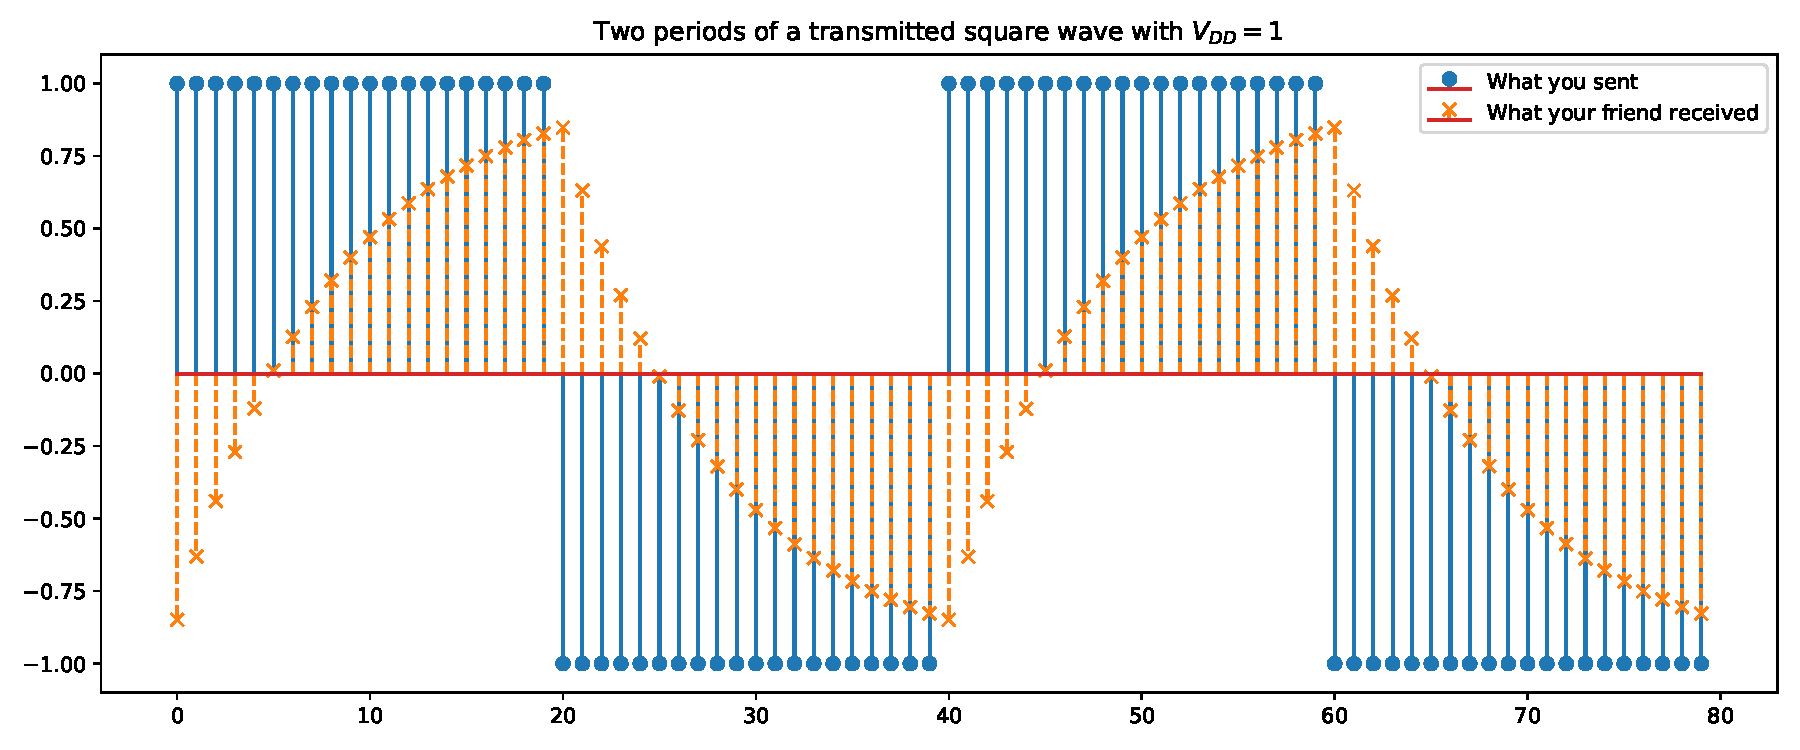
\includegraphics[width=\linewidth]{27-figs/sqwave-lowpassed}
\end{center}
What happened?
The issue is that each wire has a little bit of parasitic resistance \(R\), and there's a parasitic capacitance \(C\) between the two wires.\footnote{Especially if they stay close together.}
The time constant is \(\tau = \frac{1}{2RC}\).

\subsection{Periodic modeling}
We will express a discrete-time model at sampling interval \(T > 0\).
Let \(y[n]\) be the voltage difference at the far end of the cable at time step \(n\), and \(x[n]\) be the voltage difference at the near end.
Then the following recurrence relationship holds:
\begin{align}
  y[n+1]
  &= e^{-T/\tau} y[n] + \del{1 -e^{-T/\tau}} x[n]
  \intertext{Let's choose an even number \(N = M/2\) and send the following square wave:}
  x[n]
  &= \begin{cases}
    1, & n = 0, \ldots, M-1 \quad (\text{mod}\ N)\\
    -1, & n = M, \ldots, N-1 \quad (\text{mod}\ N)
\end{cases}
  \intertext{Therefore we use the state equation to write the following equations describing \(y[1]\) through \(y[N]\):}
  y[1] &= e^{-T/\tau} y[0] + \del{1 - e^{-T/\tau}} x[0] \notag \\
  y[2] &= e^{-T/\tau} y[1] + \del{1 - e^{-T/\tau}} x[1] \notag \\
  \vdots\phantom{[1]} &= \phantom{e^{-T\tau}} \vdots \notag \\
  y[N] &= e^{-T/\tau} y[N - 1] + \del{1 - e^{-T/\tau}} x[N - 1] \notag
  \intertext{Since \(x\) is \(N\)-periodic, so is \(y\) in steady state, so
  \(y[N] = y[0]\) and our last equation is replaced with the following.}
  y[0] &= e^{-T/\tau} y[N - 1] + \del{1 - e^{-T/\tau}} x[N - 1]
  \intertext{
  We can write all \(N\) scalar equations as a single vector equation.
  Treat \(x\) and \(y\) as sample vectors in \(\mathbb{C}^N\).
  Define a circular shift matrix \(S\) such that \((Sy)[n] = y[n+1]\).
  }
  Sy &= e^{-T/\tau} y + \del{1 - e^{-T/\tau}} x \\
  \del{S - e^{-T/\tau} I}y &= \del{1 - e^{-T/\tau}} x \\
  \intertext{We will see later that \(S\)'s eigenvalues are the \(N\)th roots of unity, so \(\del{S - e^{-T/\tau} I}\) is invertible.}
  y &= \del{1 - e^{-T/\tau}}\del{S - e^{-T/\tau} I}^{-1} x.
  \intertext{The matrix \(H \in\mathbb{R}^{n\times n}\) converts a full period of \(x[\cdot]\) to a full period of \(y[\cdot]\). On the near end of the cable \(x\) repeats forever, and on the far end \(Hx\) repeats forever. (Notice that it seems to depend only on things intrinsic to the system itself. It works for any \(x\).)}
  H &= \del{1 - e^{-T/\tau}}\del{S - e^{-T/\tau} I}^{-1}
  \intertext{We will now check that \(H\) makes sense in the cases where \(\tau\) is very small and very large. First, as \(\tau \to 0\), then \(e^{-T/\tau} \to 0\), so}
  H_\text{fast} &= \lim_{\tau \to 0} \del{1 - e^{-T/\tau}}\del{S - e^{-T/\tau} I}^{-1} = S^{-1},
  \intertext{that is, \(y[n] = x[n-1]\). The output waveform is exactly a square wave, reproduced as nearly instantaneously as our sampling interval \(T\) permits. On the other hand}
  H_\text{slow} &=
  \lim_{\tau \to \infty}
  \del{1 - e^{-T/\tau}}\del{S - e^{-T/\tau} I}^{-1} \\
  &= \lim_{\epsilon \to 0} \epsilon \del{S - (1 - \epsilon) I}^{-1}
\end{align}
which is an indeterminate ``0/0'' quotient (numerator becomes zero, and the denominator becomes singular) that I can't find an elementary way to evaluate.\footnote{Let me know if you find one.}

\subsection{In the standard basis}
Let's examine \(H\) by viewing its columns, viz.~the images of the standard basis under \(H\).
Column 0 (the first column) looks like this:
\begin{center}
  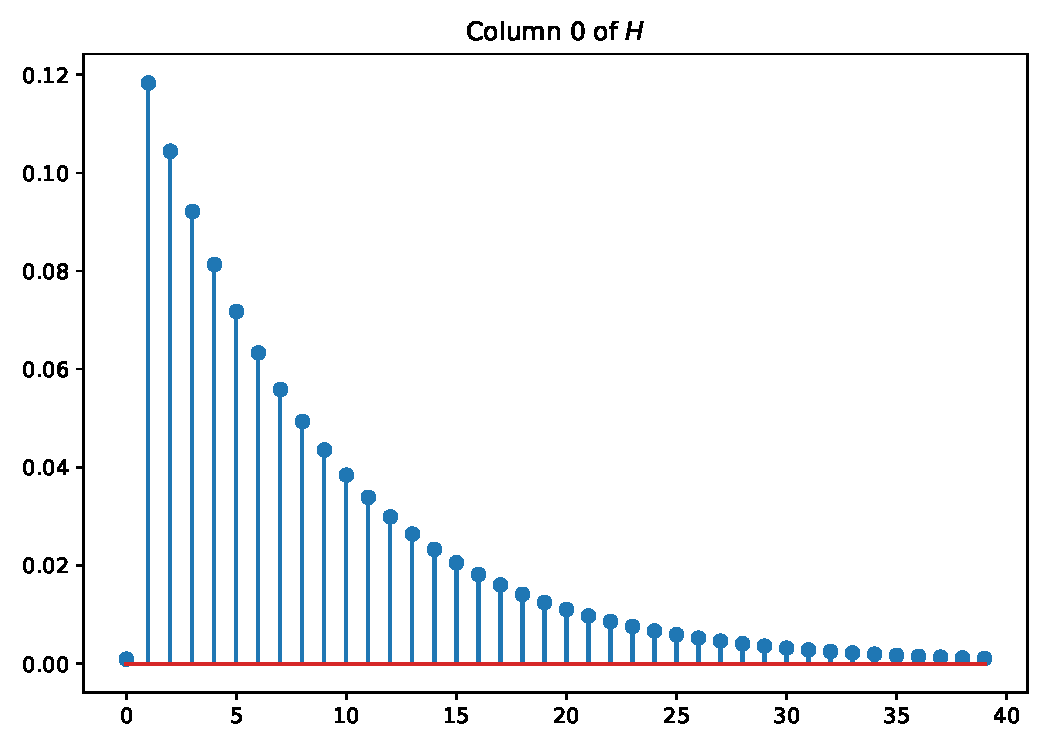
\includegraphics[width=0.618\linewidth]{27-figs/H-0}
\end{center}
and column 1 looks like this:
\begin{center}
  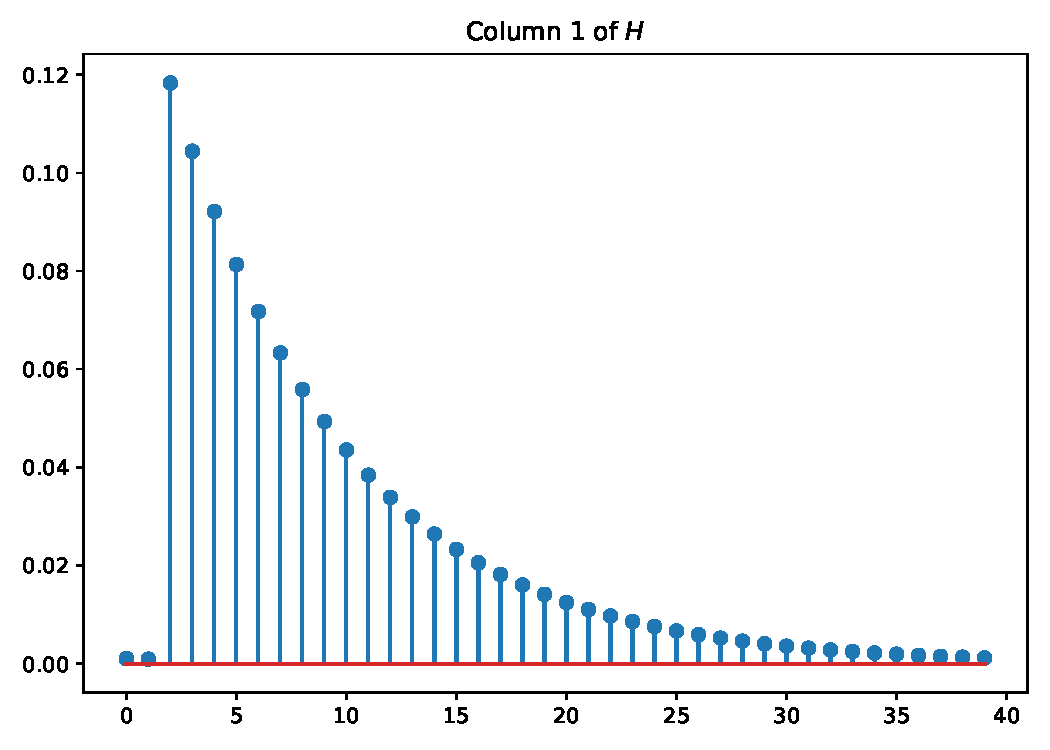
\includegraphics[width=0.618\linewidth]{27-figs/H-1}
\end{center}
You might suspect that column 1 is a right shift\footnote{That is, a right circular shift.} of column 0, and column 2 is a right shift of column 1, and so on.
That would be correct.
% We can prove it like this.
% Because of the circular symmetry of our periodic steady-state equations,
% a shift in the input corresponds to a shift in the output:
% \begin{align}
%   y &= Hx
%   \implies Sy = HSx.
%   % \intertext{We will examine the rela}
% \end{align}

\section{General discrete periodic LTI systems}
Let \(x\in\mathbb{C}^N\) represent a period of input.
Let \(y \in \mathbb{C}^N\) represent a period of input.
A \textbf{linear system} is the relationship\footnote{Lots of \texttt{textbf} ahead! These are definitions!}
\begin{align}
  y &= H x, \quad H \in \mathbb{C}^{N\times N}.
  \intertext{As above, let \(S\) represent a left shift by one sample: \((Sy)[n] = y[n+1]\). If shifts in input correspond to shifts in output, viz.}
  SH &= HS,
  \intertext{the system \(y = Hx\) is called \textbf{time-invariant}.
  Most of our systems from now on with be both linear and time-invariant.
  }
  \intertext{
  When representing periodic signals it is customary to write the standard basis 0-indexed as using the symbol \(\delta_k\) (instead of the ordinary 1-indexed \(e_k\)).}
  \delta_k[n] &=
  \begin{cases}
    1, & n = k\\
    0, & n \neq k
  \end{cases}
  \intertext{\(\delta_i\) is called an \textbf{impulse at time \(i\)}.
  Sometimes \(\delta_0\) is referred to as ``the'' impulse.
  All impulse signals are iterated shifts of \(\delta_0\):}
  \delta_i &= S^{-i} \delta_0
  \intertext{The 0th column of \(H\) is called the \textbf{impulse response} of the linear time-invariant system \(y = Hx\), and it is usually called \(h\).}
  h &= H \delta_0
\end{align}
\section{Convolution: LTI, one impulse at a time}
It is possible to express the LTI system \(y = Hx\) in terms of \(h=H\delta_0\).
Represent \(x\) as a linear combination of standard basis vectors:
\begin{align}
  y &= Hx\\
  &= H\sum_{k = 0}^{N - 1} x[k] \delta_k
  \intertext{Represent each constituent impulse as a shifted \(\delta_0\).}
  &= H\sum_{k = 0}^{N - 1} x[k] \del{S^{-k} \delta_0}\\
  % \intertext{Distribute \(H\) from the left.}
  &= \sum_{k = 0}^{N - 1} x[k] H \del{S^{-k} \delta_0}
  = \sum_{k = 0}^{N - 1} x[k] \del{H S^{-k}} \delta_0
  \intertext{Time-invariance means that \(H\) and \(S\) commute.}
  &= \sum_{k = 0}^{N - 1} x[k] \del{S^{-k} H} \delta_0
  = \sum_{k = 0}^{N - 1} x[k] S^{-k} \del{H\delta_0}\\
  &= \sum_{k = 0}^{N - 1} x[k] S^{-k} h
  \intertext{When \(x = \delta_n\), this equation verifies our earlier observation that all columns of \(H\) are right circular shifts of \(h\). Now let's make a formula for sample \(n\) of the output.}
  y[n] &= \sum_{k = 0}^{N - 1} x[k] \del{S^{-k} h}[n] \\
  &= \sum_{k = 0}^{N - 1} x[k] h[n -k]
  % \intertext{}
\end{align}
This formula is called the \textbf{circular convolution} of \(x\) with \(h\).

\chapter{Convolution and the DFT}
The DFT diagonalizes convolutions.
Throughout, let \(S \in\mathbb{C}^N\) be the left circular shift matrix defined by
% \begin{align}
  \((Sx)[n] = x[n+1]\),
  % \intertext{
  where circular indexing is understood.
% \end{align}

% \section{Eigendecomposition of circular shift}
\begin{lemma}[Eigendecomposition of circular shift]
  The eigenvectors of \(S\) are the DFT basis vectors, and that the eigenvalues are the roots of unity.\footnote{We could just verify this directly, but I find that diagonalizing \(S\) helps to clarify the magic surrounding the DFT basis.}
\end{lemma}
\begin{proof}
To show this, suppose we have an eigenvalue-eigenvector pair
\begin{align}
  Sv &= \lambda v.
  \intertext{Multiplying through by \(S^{N-1}\),}
  S^N v &= \lambda S^{N - 1} v = \lambda^2 S^{N-2} v = \ldots = \lambda^N v.
  \intertext{On the left, \(S^N = I\) as \(N\) rotations amount to a revolution.}
  v &= \lambda^N v \\
  \del{\lambda^N - 1} v &= 0
  \intertext{As \(v\) is nonzero by virtue of being an eigenvector, by the zero product property,}
  \lambda^N &= 1\\
  \lambda &= \omega_N^0, \omega_N^1, \ldots, \omega_N^{N - 1}
  \intertext{Let's solve for \(u_k\), the eigenvector corresponding to \(\omega^k\).}
  S u_k &= \omega^k u_k \\
  % \intertext{At position \(n + }
  u_k[n + 1] &= \omega^k u_k[n]
  % \intertext{This so}
\end{align}
This shows that \(u_k\) consists of consecutive powers of \(\omega^k\).
Normalizing by \(\del{\sqrt{N}}^{-1}\) we have the DFT basis.
\end{proof}

% The eigenvalues of \(S\) are the \(N\)th roots of unity are the essence of all things \(N\)-periodic.

% \section{Interlude: matrix polynomials}
A \textbf{polynomial} in the indeterminate \(z\) is an expression of the form
\(p(z) = \sum_{k = 0}^{d} p_k z^k\), where \(d \geq 0\).
When \(p(z)\) is evaluated at a matrix \(A\), we use \(A^0 = I\).
\begin{lemma}[Eigendecomposition of a matrix polynomial]
  % \tag{lemma:matpol}
  Let \(A \in\mathbb{C}^{n\times n}\), and let \(p(z)\) be a polynomial in the indeterminate \(z\).
  Then if \(Av = \lambda v\) is an eigenvalue-eigenvector pair,
  then \(p(A) v = p(\lambda) v\).
\end{lemma}
\begin{proof}
  Let \(d\) be the degree of \(p\).
  \begin{align}
    p(A) v &= \sum_{k=0}^{d} p_k A^k v\\
    \intertext{It can be shown by induction on \(k\) that \(A^k v = \lambda^k\)v.}
    p(A) v &= \sum_{k=0}^{d} p_k \lambda^k v \\
    &= \del{\sum_{k=0}^{d} p_k \lambda^k} v\\
    &= p(\lambda) v
  \end{align}
  Therefore \(p(A)\) has the same eigenvectors as \(A\), but the eigenvalues are \(p(\lambda)\) for each eigenvalue \(\lambda\) of \(A\).
\end{proof}

\subsection{Example: Cayley-Hamilton theorem}
We can use calculus to show that if \(\chi\) is the characteristic polynomial of \(A\in\mathbb{C}^{n\times n}\), then \(\chi(A) = 0\).
First, if \(A\) is diagonalizable, then for every eigenvalue-eigenvector pair
\(A v = \lambda v\), we have \(\chi(A) v = \chi(\lambda) v = 0v\).
The matrix \(\chi(A)\) annihilates the eigenvectors of \(A\), which are a basis for \(\mathbb{C}^N\). Therefore \(\chi(A) = 0\).

If \(A\) is not diagonalizable, then let \(A = U M U^*\), where \(M\) is upper triangular and \(U\) is unitary.
Let \(D\) be a diagonal matrix such that \((M+\epsilon D)\) has no repeated diagonal elements for all sufficiently small \(\epsilon > 0\).
Let \(A_\epsilon = U\del{M + \epsilon}U^*\).
Then \(\chi_A(A) = \lim_{\epsilon \to 0} \chi_{A_\epsilon}(A_\epsilon)\).
For all \(\epsilon > 0\), \(A_\epsilon\) is diagonalizable and therefore vanishes under its own characteristic polynomial.
As polynomial functions are continuous, therefore \(\chi_A(A) =0 \).
% For every \(\epi

\subsection{Example: heat equation on a ring}
Let \(x[t] \in \mathbb{R}^N\) represent the temperatures of a solid ring, sampled at evenly spaced intervals.
According to the heat equation\footnote{Solved by Fourier using a continuous-time analog of the DFT.}, \(x\) evolves according to the following law:
\begin{align}
  x[t+1] &= A x[t], \quad \text{where} \\
  A &= \frac{1}{4}(2I + S + S^{N-1}).
  \intertext{\(A\) may be written as \(p(S)\), where \(p\) is the following polynomial:}
  p(z) &= \frac{1}{4}(2 + z + z^{N-1})
  \intertext{Therefore the eigenvectors of \(A\) are the DFT basis vectors, and the eigenvalues of \(A\) are}
  p(\omega_N^k)
  &= \frac{1}{4}(2 + \omega_N^k + \omega_N^{-k}) = \frac{1}{2}\del{1 + \cos{2\pi k/N}},
\end{align}
and this system is marginally stable.


\section{\(H\) is polynomial in \(S\), and a lot of conclusions}
If \(y = Hx\) for \(x,y \in\mathbb{C}^N\) is a linear time-invariant system with impulse response \(h\),
 then \(H\) is constant along stripes parallel to the diagonal.
 Decomposing \(H\) into its \(N\) stripes,
\begin{align}
  H &= \sum_{k=0}^{N-1} h[k] S^{-k}
  \intertext{Multiplying by \(S^N = I\),}
   &= \sum_{k=0}^{N-1} h[k] S^{N -k}\\
  &= \sum_{k=0}^{N-1} h[k] S^{N -k}\\
  &= p(S),\ \text{where}\
  \ p(z) = \sum_{k=0}^{N-1} h[k] z^{N- k}.\\
  \intertext{Therefore \(H\), being a polynomial in \(S\), has the same eigenvectors as \(S\). The DFT basis vector \(u_k\) satisfies \(Su_k = \omega_N^k u_k\), so it is also an eigenvector of \(H\) with eigenvalue \(p(\omega_N^k)\):}
  H u_k &= p(\omega^k) u_k
  \intertext{Let's find out what our eigenvalue \(p(\omega^k)\) is.}
  p(\omega^k)
  &= \sum_{\ell=0}^{N-1} h[\ell] \omega^{k(N- \ell)}
  \intertext{It's row \(k\) of the DFT analysis equation! Using the DFT}
  g &= Fh,\\
  \intertext{we have}
  p(\omega^k) &= \sqrt{N} g[k].
  \intertext{Therefore \(H\) has the following eigendecomposition:}
  H
  &= F^*
   G
  F =
  F^* \operatorname{diag}\{g\} F\\
  &=
  F^*
  \begin{pmatrix}
    \sqrt{N} g[0]      &   &    \\
     & \sqrt{N}  g[1] \\
     &                 & \ddots &\\
     &                &         & \sqrt{N} g[N-1]
  \end{pmatrix}
  F.
  \intertext{In the DFT basis, time domain convolution is represented as a pointwise multiplication (using the symbol \(\odot\)).}
  Fy &= \del{\sqrt{N} Fh} \odot Fx
\end{align}
Efficient algorithms for DFT and inverse DFTs can take advantage of the fact that \(F\) and \(F^*\) are symmetric matrices.
They run as fast as an efficient sorting algorithm.

\section{Square wave transmission, revisited}
\subsection{An indeterminate matrix limit}
We derived that the convolution matrix of a transmission line with time constant \(\tau\) is
\begin{align}
  H &= \del{1 - e^{-T/\tau}} \del{S - e^{-T/\tau} I} ^{-1}.
  \intertext{We showed that as \(\tau\to0\), \(H\to S^{-1}\), a one-sample delay.
  As \(\tau\to \infty\), \(\del{1 - e^{-T/\tau}} \to 0\), we have a ``0/0'' limit.}
  H_\text{slow}
  &= \lim_{\epsilon \to 0} \epsilon \del{S - \del{1-\epsilon} I}^{-1}
  \intertext{Diagonalize \(S\) as \(S = F^* \Omega F\), where \(\Omega = \operatorname{diag}\left\{\omega_N^0, \omega_N^1, \ldots, \omega_N^{N-1}\right\}\).}
  &= \lim_{\epsilon \to 0} \epsilon \del{F^*\Omega F - \del{1-\epsilon} I}^{-1}\\
  &= \lim_{\epsilon \to 0}
  \epsilon \del{F^*\del{\Omega  - \del{1-\epsilon} I}F}^{-1} \\
  &= \lim_{\epsilon \to 0}
  F^*\del{\frac{\Omega  - \del{1-\epsilon} I}{\epsilon}}^{-1}F \\
  &= \lim_{\epsilon \to 0}
  F^*
  \operatorname{diag}\left\{
    \frac{\epsilon}{\omega_N^0 - 1 + \epsilon},
    \frac{\epsilon}{\omega_N^1 - 1 + \epsilon}, \ldots,
    \frac{\epsilon}{\omega_N^{N-1} - 1 + \epsilon}
  \right\}
  F \\
  &= \lim_{\epsilon \to 0}
  F^*
  \operatorname{diag}\left\{
    \frac{\epsilon}{\epsilon},
    \frac{\epsilon}{\del{\text{nonzero}}}, \ldots,
    \frac{\epsilon}{\del{\text{nonzero}}}
  \right\}
  F \\
  &=
  F^*
  \operatorname{diag}\left\{1, 0, \ldots, 0 \right\}
  F \\
  &=
  \frac{1}{N}
  \begin{pmatrix}
    1 & \cdots & 1 \\
    \vdots & \ddots & \vdots \\
    1 & \cdots & 1 \\
  \end{pmatrix}
\end{align}
As our transmission line becomes infinitely slow, eventually it becomes impossible to move the output at all, and all AC signals are shorted through the parasitic shunt capacitor.
Only the DC component of the input passes.

\subsection{Input, transfer function, output}

\begin{figure}
  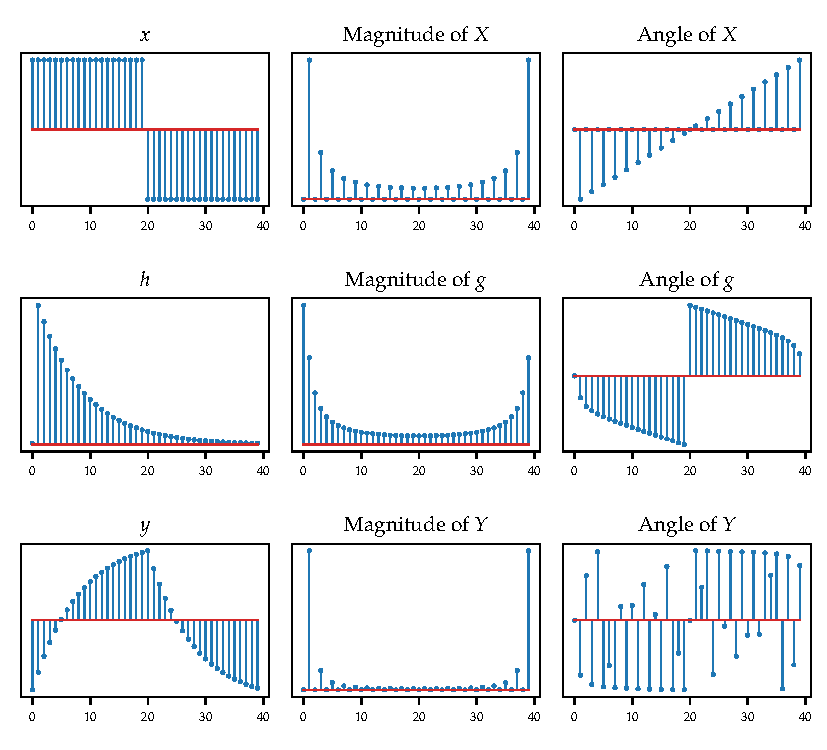
\includegraphics{27-figs/inHout}
  \caption{Input, impulse response, and output in time and frequency domain.}
  \label{fig:lec27-inHout}
\end{figure}
The left column of Figure~\ref{fig:lec27-inHout} shows:
\begin{itemize}
  \item \(x\), the square wave on the near end of the transmission line;
  \item \(h\), the impulse response of the transmission line; and
  \item \(y\), the output on the far end of the transmission line.
\end{itemize}
We showed that \(y\) is the convolution of \(x\) with \(h\).

The center and right columns of Figure~\ref{fig:lec27-inHout} show:
\begin{itemize}
  \item \(X= Fx\), the ``phasor'' representation of \(x\) in the DFT basis (note that \(x\) has only odd frequencies);
  \item \(g = Fx\), the ``transfer function'' representation of \(h\) in the DFT basis (can you tell that \(g\) is a low-pass filter?); and
  \item \(Y = \sqrt{N} g \odot X\), the ``phasor'' representation of \(y\) in the DFT basis. (When eyeballing \(g \odot X\), remember that magnitudes multiply and phases add.)\footnote{The phase of \(Y\) is crazy; don't think too hard about what it means.}
\end{itemize}

\subsection{Equalization using DFT}
\begin{figure}
  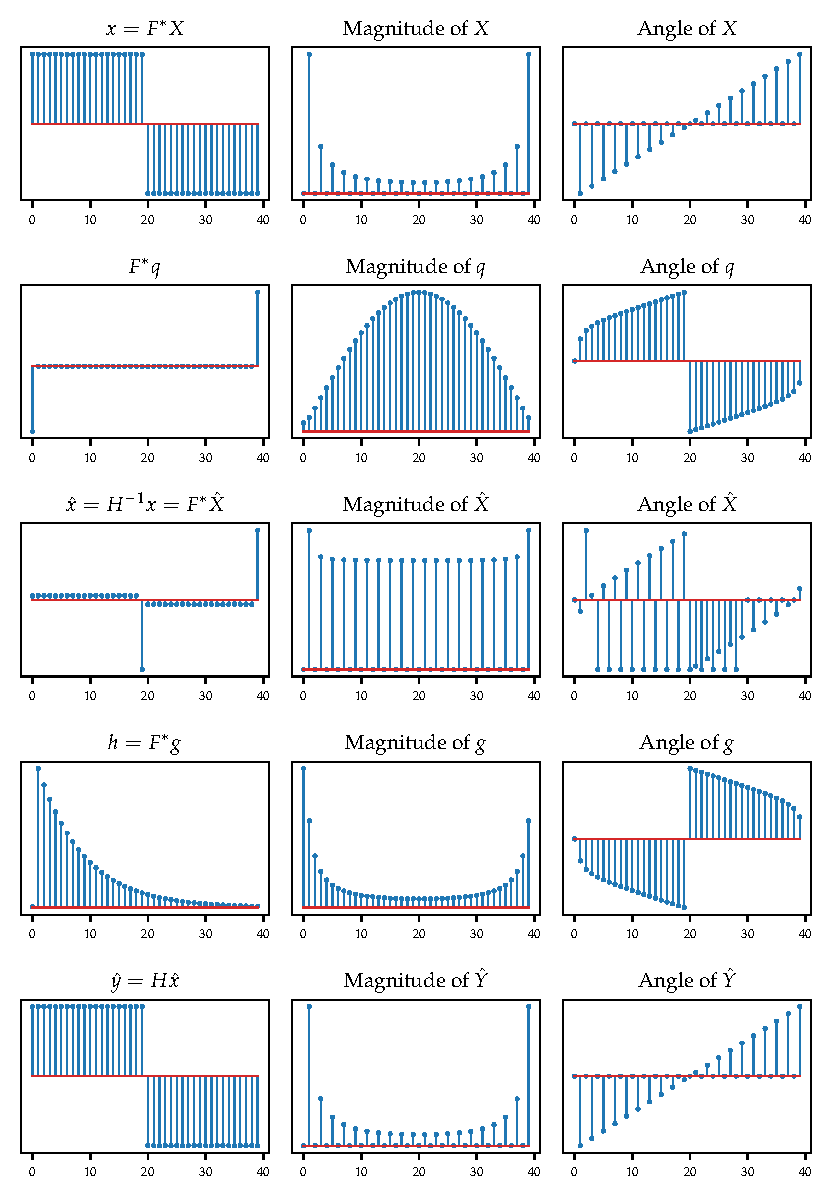
\includegraphics{27-figs/eq}
  \caption{Input, impulse response, and output in time and frequency domain.}
  \label{fig:lec27-eq}
\end{figure}

The transmission equation
\begin{align}
  y &= Hx \\
  \intertext{has the frequency domain representation}
  Y &= \sqrt{N} g \odot X,
  \intertext{where \(Y = Fy\), \(g = Fh\), and \(X = Fx\). To achieve a square wave output, we can cancel \(\sqrt{N}g\) by pre-dividing by \(\sqrt{N}g\). That is, define a frequency response \(q\) by}
  q[n] &= \frac{1}{\sqrt{N}g[n]},
  \intertext{then define our pre-equalized input \(\hat X\) in frequency domain by}
  \hat X &= q[n] \odot X,
  \intertext{resulting in}
  \hat Y &= \sqrt{N} g \odot \hat X = \sqrt{N} g\odot \del{q \odot X} = X
\end{align}
Therefore \(F^* \hat X\) is what you should send in order to make sure your friend across the lab receives the square wave \(X\).
Figure~\ref{fig:lec27-eq} shows the pre-equalized input, equalization filter, equalized input, transmission filter, and output.
Observe that equalization is the inverse of transmission.


\end{document}
